
\documentclass[11pt,a4paper,oneside]{report}
\usepackage[T1]{fontenc}
\usepackage[utf8]{inputenc}
\usepackage{lmodern}
\usepackage{microtype}
\usepackage[a4paper,margin=22mm,headheight=16pt]{geometry}
\usepackage{xcolor}
\definecolor{BankNavy}{HTML}{09213A}
\definecolor{BankTeal}{HTML}{159D91}
\definecolor{BankGold}{HTML}{C79A45}
\definecolor{SoftGray}{HTML}{F2F5F8}
\definecolor{CodeBg}{HTML}{F7F9FB}
\usepackage{graphicx}
\usepackage{booktabs}
\usepackage{longtable}
\usepackage{tabularx}
\usepackage{array}
\usepackage{ragged2e}
\usepackage{pdflscape}
\usepackage{enumitem}
\setlist{nosep,leftmargin=1.4em}
\usepackage{tikz}
\usetikzlibrary{arrows.meta,positioning,fit,shapes.geometric,calc}
\usepackage[most]{tcolorbox}
\usepackage{listings}
\usepackage{fancyhdr}
\usepackage{titlesec}
\usepackage{xurl}
\usepackage{hyperref}
\hypersetup{colorlinks=true,linkcolor=BankTeal,urlcolor=BankTeal,citecolor=BankTeal,pdftitle={BankManagement Technical Report}}
\usepackage{bookmark}
\usepackage{caption}
\usepackage{float}
\usepackage{multicol}
\usepackage{makecell}
\usepackage{lastpage}
\usepackage{amsmath}
\usepackage{amssymb}
\usepackage{etoolbox}
\usepackage{setspace}
\setstretch{1.08}
\raggedbottom
\setlength{\tabcolsep}{3pt}
\setlength{\LTleft}{0pt}
\setlength{\LTright}{0pt}
\setlength{\LTpre}{5pt}
\setlength{\LTpost}{8pt}
\setlength{\LTcapwidth}{\textwidth}
\AtBeginEnvironment{longtable}{\small\renewcommand{\arraystretch}{1.12}}
\urlstyle{tt}

\pagestyle{fancy}
\fancyhf{}
\fancyhead[L]{\small\textcolor{BankNavy}{BankManagement}}
\fancyhead[R]{\scriptsize\textcolor{BankTeal}{\leftmark}}
\fancyfoot[C]{\thepage\ / \pageref{LastPage}}
\renewcommand{\headrulewidth}{0.4pt}
\renewcommand{\footrulewidth}{0pt}

\titleformat{\chapter}[display]{\bfseries\color{BankNavy}\RaggedRight}{\Large Chapter \thechapter}{6pt}{\LARGE}
\titleformat{\section}{\Large\bfseries\color{BankNavy}}{\thesection}{0.6em}{}
\titleformat{\subsection}{\large\bfseries\color{BankTeal}}{\thesubsection}{0.6em}{}

\newtcolorbox{defensebox}[1][]{enhanced,breakable,colback=SoftGray,colframe=BankTeal,boxrule=0.7pt,arc=2mm,title=#1,fonttitle=\bfseries\color{BankNavy}}
\newtcolorbox{warningbox}[1][]{enhanced,breakable,colback=yellow!7,colframe=BankGold,boxrule=0.7pt,arc=2mm,title=#1,fonttitle=\bfseries\color{BankNavy}}
\newcommand{\codepath}[1]{\nolinkurl{#1}}
\newcommand{\apipath}[1]{\texttt{#1}}
\newcommand{\sqlobj}[1]{\texttt{#1}}
\newcommand{\role}[1]{\textsf{#1}}
\newcolumntype{L}[1]{>{\RaggedRight\arraybackslash}p{#1}}
\newcolumntype{Y}{>{\RaggedRight\arraybackslash}X}
\newcolumntype{C}[1]{>{\Centering\arraybackslash}p{#1}}

\lstdefinestyle{bankcode}{backgroundcolor=\color{CodeBg},basicstyle=\ttfamily\footnotesize,breaklines=true,frame=single,rulecolor=\color{BankTeal!45},numbers=left,numberstyle=\tiny\color{gray},showstringspaces=false,tabsize=2,columns=fullflexible}
\lstset{style=bankcode}

\emergencystretch=3em
\lstdefinelanguage{JavaScript}{
  keywords={const,let,var,function,return,async,await,if,else,for,of,new,throw,try,catch,class,extends,true,false,null,undefined},
  sensitive=true,
  comment=[l]{//},
  morecomment=[s]{/*}{*/},
  morestring=[b]',
  morestring=[b]"
}
\lstdefinelanguage{Bash}{
  keywords={cd,npm,node,export,set,echo},
  sensitive=true,
  comment=[l]{\#},
  morestring=[b]',
  morestring=[b]"
}

\begin{document}
\begin{titlepage}
\pagecolor{BankNavy}
\color{white}
\vspace*{14mm}
{\Huge\bfseries BankManagement\\[3mm]}
{\LARGE Database and Software Architecture Report\\[7mm]}
\textcolor{BankTeal!45!white}{\rule{\textwidth}{1.2pt}}\\[10mm]
{\Large Design, Implementation, Security, and System Integration}

\vspace{18mm}
\begin{tcolorbox}[
  colback=BankNavy!72!black,
  colframe=BankTeal,
  boxrule=0.9pt,
  arc=3mm,
  left=5mm,right=5mm,top=4mm,bottom=4mm
]
\color{white}
\textbf{Technology stack}\\
Microsoft SQL Server and T-SQL; Node.js and Express; the \texttt{mssql} SQL Server driver; vanilla HTML, CSS, and JavaScript.\\[3mm]
\textbf{Implementation approach}\\
The database contains the main business rules through tables, keys, constraints, stored procedures, functions, triggers, views, database roles, and Agent jobs. The backend calls these SQL objects directly; it does not use an object-relational mapper.
\end{tcolorbox}

\vfill
\begin{tabular}{@{}ll@{}}
\textbf{Student:} & \rule{85mm}{0.4pt}\\[4mm]
\textbf{Course:} & Database Systems\\[4mm]
\textbf{Instructor:} & \rule{78mm}{0.4pt}\\[4mm]
\textbf{Date:} & \rule{91mm}{0.4pt}
\end{tabular}
\vspace*{10mm}
\end{titlepage}
\nopagecolor
\color{black}
\pagenumbering{roman}
\chapter*{Executive Summary}
\addcontentsline{toc}{chapter}{Executive Summary}
This report describes the design and implementation of the BankManagement project. The main emphasis is the SQL Server database: the relational schema, integrity rules, stored procedures, views, triggers, functions, security roles, reports, audit records, and scheduled jobs. The report also explains how the Node.js/Express API communicates with SQL Server and how the browser interface uses the API.

The current implementation contains seventeen relational tables, fifty-two stored procedures, fifteen reporting and helper views, six integrity triggers, two scalar functions, five database-security personas, and three SQL Server Agent jobs. Application identities are separate from SQL Server logins. The application uses four effective roles: Customer, Employee, Admin, and HighAdmin. A stored role is not accepted by itself; the session-validation procedure also checks the current customer status, employee status, job title, administrative capability, and active branch assignment.

\begin{defensebox}[System path in one line]
Browser interface $\rightarrow$ Express route $\rightarrow$ session and role middleware $\rightarrow$ typed \texttt{mssql} parameters $\rightarrow$ stored procedure or protected view $\rightarrow$ SQL Server rules and audit $\rightarrow$ JSON response $\rightarrow$ role-aware interface.
\end{defensebox}

\tableofcontents
\listoftables
\listoffigures
\clearpage
\pagenumbering{arabic}

\chapter{Project Scope and Requirements}
\section{Problem statement}
The system models a multi-branch bank in which customers may own accounts at different branches, staff work through temporal branch assignments, financial operations are queued and finalized safely, loans are divided into installments, and access is controlled by both application roles and database-level permissions.

\section{Assignment requirements and implementation mapping}
\begin{longtable}{L{0.24\textwidth}L{0.70\textwidth}}
\caption{Requirement-to-implementation mapping}\label{tab:reqmap}\\
\toprule
\textbf{Requirement} & \textbf{Implementation}\\
\midrule\endfirsthead
\toprule\textbf{Requirement} & \textbf{Implementation}\\\midrule\endhead
Relational database & SQL Server schema with normalized entity, lookup, bridge, workflow, and audit tables.\\
ER diagram and relational schema & Explicit PK/FK relationships, cardinalities, and temporal bridges documented in Chapters 3--5.\\
Customer management & Create, search, update, soft deactivate; staff results are branch scoped through customer accounts.\\
Account management & Self-service opening, visibility scopes, freeze/unfreeze, type change, close, dormant sweep, monthly interest.\\
Transactions & Owner-only deposit, withdrawal, transfer, finalization, cancellation/reversal; pending queue and batch processing.\\
Loans/installments & Branch loan creation, scoped viewing, borrower-only payment, overdue processing by branch manager or HighAdmin.\\
Employee management & Hiring, login creation, titles, suspension, termination, temporal branch history, transfers, manager governance.\\
Authentication & Username/password login, SHA2-256 password comparison, opaque server-side session token.\\
Authorization & Effective roles, branch scope, ownership checks, database procedure checks, route middleware, SQL Server roles.\\
SQL injection defense & Parameter binding through \texttt{request.input}; stored procedures; report identifiers chosen from server whitelist only.\\
No ORM & Direct \texttt{mssql} driver calls, explicit SQL types, explicit stored-procedure names, and SQL-owned business logic.\\
Audit/logging & \texttt{AuditLog}, safe audit view, branch ledger, login/logout/expiry and business-operation audit actions.\\
Session management & Server-side \texttt{Sessions} table with fixed ten-minute \texttt{ExpiresAt} and explicit revocation.\\
Responsive interface & Separate role-aware workspaces with responsive CSS, dynamic forms, dropdown catalogues, and mobile layout.\\
Reporting & Fourteen API reports backed by controlled views, separate SQL pools, paging, newest-first ordering, branch scoping, and CSV export.\\
\bottomrule
\end{longtable}

\chapter{System Architecture}
\section{Layered architecture}
\begin{figure}[H]
\centering
\resizebox{\textwidth}{!}{%
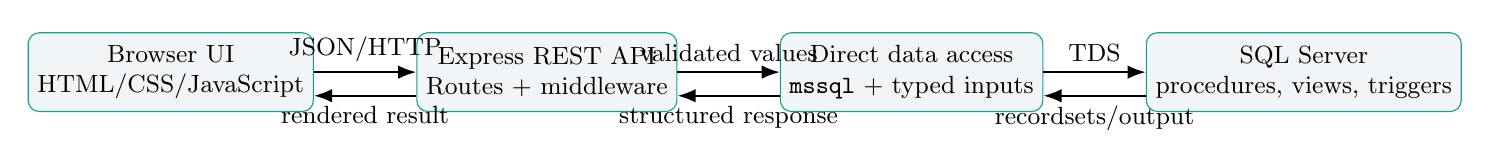
\begin{tikzpicture}[node distance=9mm and 13mm,>=Latex, every node/.style={font=\small}, box/.style={draw=BankTeal,rounded corners,fill=SoftGray,minimum width=33mm,minimum height=10mm,align=center}]
\node[box] (browser) {Browser UI\\HTML/CSS/JavaScript};
\node[box,right=of browser] (api) {Express REST API\\Routes + middleware};
\node[box,right=of api] (dal) {Direct data access\\\texttt{mssql} + typed inputs};
\node[box,right=of dal] (db) {SQL Server\\procedures, views, triggers};
\draw[->,thick] (browser) -- node[above]{JSON/HTTP} (api);
\draw[->,thick] (api) -- node[above]{validated values} (dal);
\draw[->,thick] (dal) -- node[above]{TDS} (db);
\draw[<-,thick] ([yshift=-3mm]browser.east) -- node[below]{rendered result} ([yshift=-3mm]api.west);
\draw[<-,thick] ([yshift=-3mm]api.east) -- node[below]{structured response} ([yshift=-3mm]dal.west);
\draw[<-,thick] ([yshift=-3mm]dal.east) -- node[below]{recordsets/output} ([yshift=-3mm]db.west);
\end{tikzpicture}%
}
\caption{End-to-end architecture}
\end{figure}

\section{Responsibility boundaries}
\begin{itemize}
\item \textbf{Frontend:} presentation, user input, client-side convenience validation, token storage, calling APIs, rendering role-specific sections, formatting dates, and exporting visible report data.
\item \textbf{Backend:} HTTP routing, required-field validation, bearer-token extraction, application-role checks, branch/ownership prechecks, SQL type binding, response normalization, CORS, rate limiting, and error translation.
\item \textbf{Database:} source of truth for identity, effective roles, business rules, referential integrity, transactional consistency, locking, balance changes, installment state, audit records, reporting views, and scheduled maintenance.
\end{itemize}

\section{Ports and CORS}
The frontend static server normally listens on \texttt{127.0.0.1:5500}; the backend listens on \texttt{127.0.0.1:4000}; SQL Server normally listens on port 1433. Different ports are different browser origins, so the backend allows only configured frontend origins through \texttt{CORS\_ORIGIN}. CORS is a browser boundary and is not a substitute for authentication or authorization.

\chapter{Database Conceptual and Relational Design}
\section{Core banking ER model}
\begin{landscape}
\begin{figure}[H]
\centering
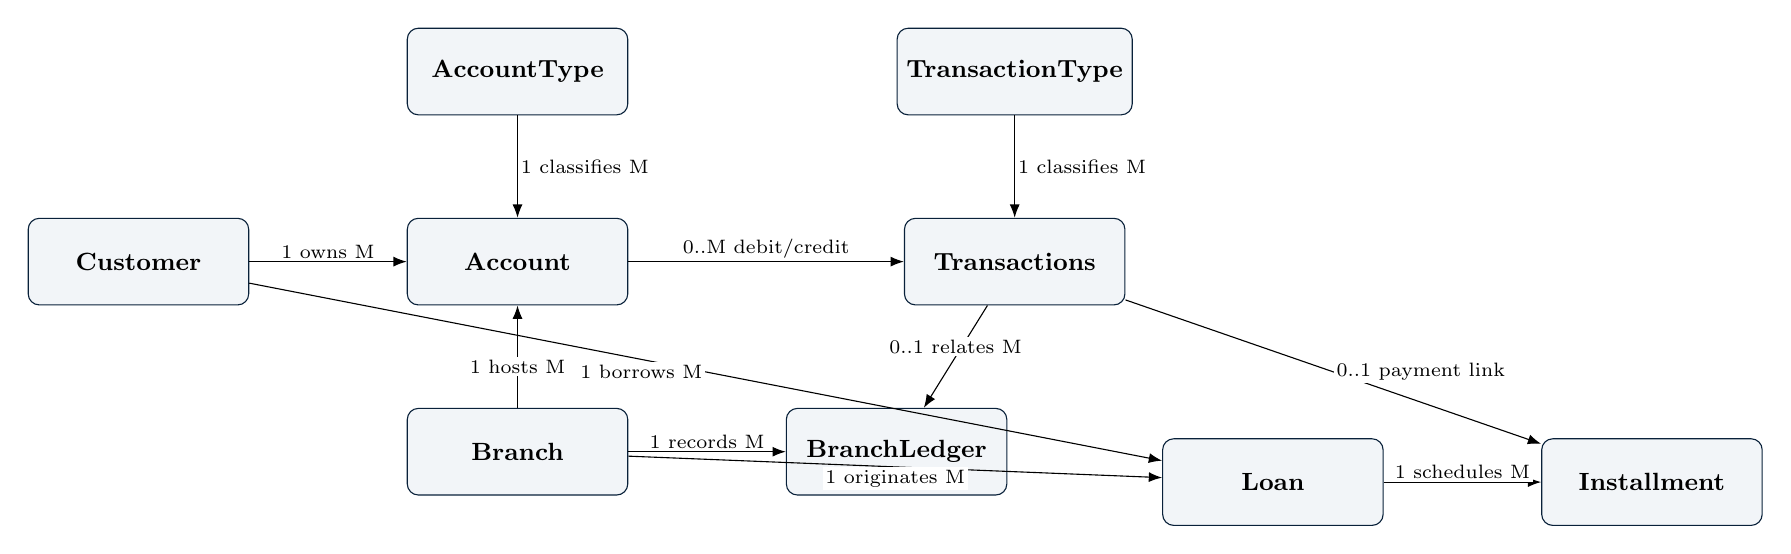
\begin{tikzpicture}[node distance=13mm and 20mm,>=Latex,
entity/.style={draw=BankNavy,rounded corners,fill=SoftGray,minimum width=28mm,minimum height=11mm,align=center,font=\small\bfseries},
rel/.style={font=\scriptsize,fill=white,inner sep=1pt}]
\node[entity] (customer) {Customer};
\node[entity,right=of customer] (account) {Account};
\node[entity,above=of account] (atype) {AccountType};
\node[entity,below=of account] (branch) {Branch};
\node[entity,right=35mm of account] (trans) {Transactions};
\node[entity,above=of trans] (ttype) {TransactionType};
\node[entity,right=35mm of customer] (loan) at ($(customer)+(95mm,-28mm)$) {Loan};
\node[entity,right=of loan] (inst) {Installment};
\node[entity,right=of branch] (ledger) {BranchLedger};
\draw[->] (customer) -- node[rel,above]{1 owns M} (account);
\draw[->] (branch) -- node[rel,below]{1 hosts M} (account);
\draw[->] (atype) -- node[rel,right]{1 classifies M} (account);
\draw[->] (account) -- node[rel,above]{0..M debit/credit} (trans);
\draw[->] (ttype) -- node[rel,right]{1 classifies M} (trans);
\draw[->] (customer) -- node[rel,left]{1 borrows M} (loan);
\draw[->] (branch) -- node[rel,below]{1 originates M} (loan);
\draw[->] (loan) -- node[rel,above]{1 schedules M} (inst);
\draw[->] (trans) -- node[rel,right]{0..1 payment link} (inst);
\draw[->] (branch) -- node[rel,above]{1 records M} (ledger);
\draw[->] (trans) -- node[rel,above]{0..1 relates M} (ledger);
\end{tikzpicture}
\caption{Core banking relationships}
\end{figure}
\end{landscape}

\section{Identity, role, and workforce ER model}
\begin{landscape}
\begin{figure}[H]
\centering
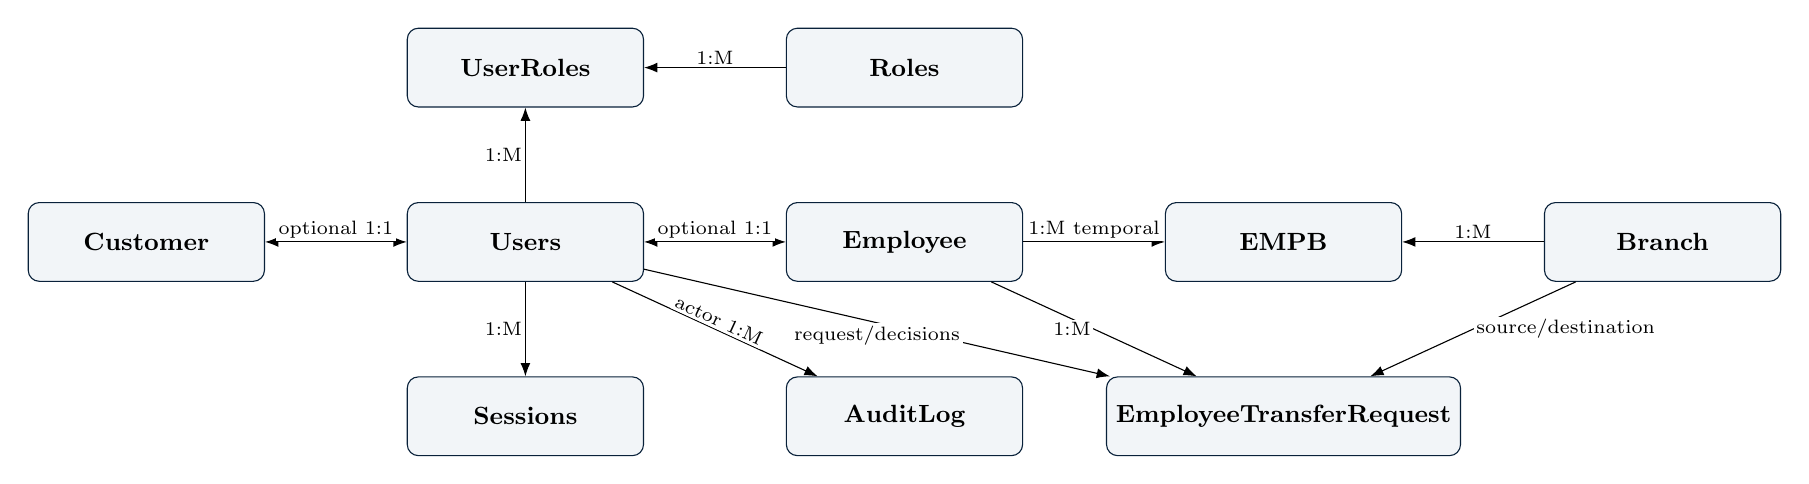
\begin{tikzpicture}[node distance=12mm and 18mm,>=Latex,
entity/.style={draw=BankNavy,rounded corners,fill=SoftGray,minimum width=30mm,minimum height=10mm,align=center,font=\small\bfseries},
rel/.style={font=\scriptsize,fill=white,inner sep=1pt}]
\node[entity] (cust) {Customer};
\node[entity,right=of cust] (users) {Users};
\node[entity,right=of users] (emp) {Employee};
\node[entity,above=of users] (ur) {UserRoles};
\node[entity,right=of ur] (roles) {Roles};
\node[entity,below=of users] (sess) {Sessions};
\node[entity,below=of emp] (audit) {AuditLog};
\node[entity,right=of emp] (empb) {EMPB};
\node[entity,right=of empb] (branch) {Branch};
\node[entity,below=of empb] (etr) {EmployeeTransferRequest};
\draw[<->] (cust) -- node[rel,above]{optional 1:1} (users);
\draw[<->] (users) -- node[rel,above]{optional 1:1} (emp);
\draw[->] (users) -- node[rel,left]{1:M} (ur);
\draw[->] (roles) -- node[rel,above]{1:M} (ur);
\draw[->] (users) -- node[rel,left]{1:M} (sess);
\draw[->] (users) -- node[rel,sloped,above]{actor 1:M} (audit);
\draw[->] (emp) -- node[rel,above]{1:M temporal} (empb);
\draw[->] (branch) -- node[rel,above]{1:M} (empb);
\draw[->] (emp) -- node[rel,left]{1:M} (etr);
\draw[->] (branch) -- node[rel,right]{source/destination} (etr);
\draw[->] (users) -- node[rel,below]{request/decisions} (etr);
\end{tikzpicture}
\caption{Application identity, roles, workforce, and transfer workflow}
\end{figure}
\end{landscape}

\section{Normalization to third normal form}
\begin{itemize}
\item Repeating descriptive values are moved to lookup tables: \texttt{AccountType}, \texttt{TransactionType}, and \texttt{Roles}.
\item Many-to-many relationships are decomposed into associative tables: \texttt{UserRoles} and temporal \texttt{EMPB}.
\item Customer, employee, user, account, loan, and branch facts are stored once under their own keys, avoiding update anomalies.
\item Loan installments are separate from Loan because each loan has a repeating schedule.
\item Transaction debit and credit references are foreign keys rather than embedded account data.
\item \texttt{Branch.Balance} and \texttt{BranchLedger} are intentional controlled denormalizations: the former is a cached aggregate and the latter is an audit history. Their consistency is centralized in a trigger.
\end{itemize}

\chapter{Complete Data Dictionary}
The following data dictionary is based on the current database schema used by the application.

\section{Customer}
Bank customer master data; soft-deleted through IsActive.
\begin{longtable}{L{0.21\textwidth}L{0.18\textwidth}L{0.24\textwidth}L{0.31\textwidth}}
\toprule
\textbf{Column} & \textbf{Type} & \textbf{Constraint/key} & \textbf{Meaning}\\
\midrule\endfirsthead
\toprule\textbf{Column} & \textbf{Type} & \textbf{Constraint/key} & \textbf{Meaning}\\\midrule\endhead
CustomerID & INT IDENTITY & NOT NULL, PK & Surrogate customer identifier.\\
FirstName & NVARCHAR(50) & NOT NULL & Given name.\\
LastName & NVARCHAR(50) & NOT NULL & Family name.\\
NationalID & NVARCHAR(20) & NOT NULL, UNIQUE, CHECK & Exactly 10 numeric digits.\\
BirthDate & DATE & NOT NULL & Date of birth; customer-creation procedures enforce adulthood.\\
Phone & NVARCHAR(20) & NOT NULL, UNIQUE & Primary telephone number.\\
Email & NVARCHAR(100) & NOT NULL, UNIQUE & Primary email address.\\
Address & NVARCHAR(200) & NULL & Postal address.\\
RegistrationDate & DATE & NOT NULL, DEFAULT today & Registration date.\\
IsActive & BIT & NOT NULL, DEFAULT 1 & Soft-deletion / active-profile flag.\\
\bottomrule
\end{longtable}

\section{Branch}
Bank branch master data and a trigger-maintained aggregate balance.
\begin{longtable}{L{0.21\textwidth}L{0.18\textwidth}L{0.24\textwidth}L{0.31\textwidth}}
\toprule
\textbf{Column} & \textbf{Type} & \textbf{Constraint/key} & \textbf{Meaning}\\
\midrule\endfirsthead
\toprule\textbf{Column} & \textbf{Type} & \textbf{Constraint/key} & \textbf{Meaning}\\\midrule\endhead
BranchID & INT IDENTITY & NOT NULL, PK & Surrogate branch identifier.\\
BranchName & NVARCHAR(100) & NOT NULL & Human-readable branch name.\\
BranchCode & NVARCHAR(20) & NOT NULL, UNIQUE & Short operational branch code.\\
Balance & DECIMAL(18,2) & NOT NULL, DEFAULT 0 & Aggregate of account-balance changes, maintained by trigger.\\
City & NVARCHAR(50) & NOT NULL & Branch city.\\
Address & NVARCHAR(200) & NULL & Branch address.\\
Phone & NVARCHAR(20) & NULL & Branch phone.\\
\bottomrule
\end{longtable}

\section{AccountType}
Lookup for account products and product rules.
\begin{longtable}{L{0.21\textwidth}L{0.18\textwidth}L{0.24\textwidth}L{0.31\textwidth}}
\toprule
\textbf{Column} & \textbf{Type} & \textbf{Constraint/key} & \textbf{Meaning}\\
\midrule\endfirsthead
\toprule\textbf{Column} & \textbf{Type} & \textbf{Constraint/key} & \textbf{Meaning}\\\midrule\endhead
AccountTypeID & INT IDENTITY & NOT NULL, PK & Account-product identifier.\\
TypeName & NVARCHAR(50) & NOT NULL, UNIQUE & Product name.\\
Description & NVARCHAR(200) & NULL & Product description.\\
MinBalance & DECIMAL(18,2) & NOT NULL, DEFAULT 0 & Minimum allowed balance.\\
InterestRate & DECIMAL(5,2) & NOT NULL, DEFAULT 0 & Monthly interest percentage used by maintenance procedure.\\
MonthlyFee & DECIMAL(18,2) & NOT NULL, DEFAULT 0 & Configured product fee (present in schema for policy use).\\
\bottomrule
\end{longtable}

\section{Account}
Customer account at one branch and of one account type.
\begin{longtable}{L{0.21\textwidth}L{0.18\textwidth}L{0.24\textwidth}L{0.31\textwidth}}
\toprule
\textbf{Column} & \textbf{Type} & \textbf{Constraint/key} & \textbf{Meaning}\\
\midrule\endfirsthead
\toprule\textbf{Column} & \textbf{Type} & \textbf{Constraint/key} & \textbf{Meaning}\\\midrule\endhead
AccountID & INT IDENTITY & NOT NULL, PK & Surrogate account identifier.\\
AccountNumber & NVARCHAR(30) & NOT NULL, UNIQUE, CHECK & Exactly 12 numeric digits; generated from sequence.\\
CustomerID & INT & NOT NULL, FK -> Customer & Account owner.\\
BranchID & INT & NOT NULL, FK -> Branch & Owning branch.\\
AccountTypeID & INT & NOT NULL, FK -> AccountType & Product type.\\
Balance & DECIMAL(18,2) & NOT NULL, DEFAULT 0 & Posted balance; pending outgoing amounts are subtracted separately for available balance.\\
OpenDate & DATE & NOT NULL & Opening date.\\
CloseDate & DATE & NULL, CHECK & Must be null or on/after OpenDate.\\
AccountStatus & NVARCHAR(20) & NOT NULL, CHECK & Active, Closed, Frozen, or Dormant.\\
FrozenPreviousStatus & NVARCHAR(20) & NULL, CHECK & Stores Active/Dormant state for unfreeze restoration.\\
\bottomrule
\end{longtable}

\section{Employee}
Personnel master data.
\begin{longtable}{L{0.21\textwidth}L{0.18\textwidth}L{0.24\textwidth}L{0.31\textwidth}}
\toprule
\textbf{Column} & \textbf{Type} & \textbf{Constraint/key} & \textbf{Meaning}\\
\midrule\endfirsthead
\toprule\textbf{Column} & \textbf{Type} & \textbf{Constraint/key} & \textbf{Meaning}\\\midrule\endhead
EmployeeID & INT IDENTITY & NOT NULL, PK & Surrogate employee identifier.\\
NationalID & NVARCHAR(20) & NOT NULL, UNIQUE & Employee national identifier.\\
FirstName & NVARCHAR(50) & NOT NULL & Given name.\\
LastName & NVARCHAR(50) & NOT NULL & Family name.\\
HireDate & DATE & NOT NULL & Hire date.\\
JobTitle & NVARCHAR(100) & NOT NULL & Operational title; manager titles are special.\\
Salary & DECIMAL(18,2) & NOT NULL & Salary.\\
Phone & NVARCHAR(20) & NULL & Employee phone.\\
Email & NVARCHAR(100) & NULL & Employee email.\\
EmpStatus & NVARCHAR(20) & NOT NULL, CHECK & Active, OnLeave, or Terminated.\\
CanAccessAdmin & BIT & NOT NULL, DEFAULT 0 & Additional gate for effective Admin privilege.\\
\bottomrule
\end{longtable}

\section{EMPB}
Temporal employee-to-branch assignment bridge.
\begin{longtable}{L{0.21\textwidth}L{0.18\textwidth}L{0.24\textwidth}L{0.31\textwidth}}
\toprule
\textbf{Column} & \textbf{Type} & \textbf{Constraint/key} & \textbf{Meaning}\\
\midrule\endfirsthead
\toprule\textbf{Column} & \textbf{Type} & \textbf{Constraint/key} & \textbf{Meaning}\\\midrule\endhead
EMPBID & INT IDENTITY & NOT NULL, PK & Assignment identifier.\\
EmployeeID & INT & NOT NULL, FK -> Employee & Assigned employee.\\
BranchID & INT & NOT NULL, FK -> Branch & Assigned branch.\\
StartDate & DATE & NOT NULL & Assignment start.\\
EndDate & DATE & NULL, CHECK & Null while current; otherwise not earlier than StartDate.\\
WorkingStatus & NVARCHAR(20) & NOT NULL, CHECK & Working, Transferred, or Ended.\\
\bottomrule
\end{longtable}

\section{TransactionType}
Lookup for transaction semantics.
\begin{longtable}{L{0.21\textwidth}L{0.18\textwidth}L{0.24\textwidth}L{0.31\textwidth}}
\toprule
\textbf{Column} & \textbf{Type} & \textbf{Constraint/key} & \textbf{Meaning}\\
\midrule\endfirsthead
\toprule\textbf{Column} & \textbf{Type} & \textbf{Constraint/key} & \textbf{Meaning}\\\midrule\endhead
TransactionTypeID & INT IDENTITY & NOT NULL, PK & Transaction-type identifier.\\
TypeName & NVARCHAR(50) & NOT NULL, UNIQUE & Deposit, Withdrawal, Transfer, or Interest.\\
\bottomrule
\end{longtable}

\section{Transactions}
Financial transaction queue and history.
\begin{longtable}{L{0.21\textwidth}L{0.18\textwidth}L{0.24\textwidth}L{0.31\textwidth}}
\toprule
\textbf{Column} & \textbf{Type} & \textbf{Constraint/key} & \textbf{Meaning}\\
\midrule\endfirsthead
\toprule\textbf{Column} & \textbf{Type} & \textbf{Constraint/key} & \textbf{Meaning}\\\midrule\endhead
TransactionID & INT IDENTITY & NOT NULL, PK & Transaction identifier.\\
TransactionTypeID & INT & NOT NULL, FK -> TransactionType & Transaction semantic type.\\
FromAccountID & INT & NULL, FK -> Account & Debit account, where applicable.\\
ToAccountID & INT & NULL, FK -> Account & Credit account, where applicable.\\
EmployeeID & INT & NULL, FK -> Employee & Optional staff metadata; must match authenticated employee when supplied.\\
Amount & DECIMAL(18,2) & NOT NULL, CHECK > 0 & Monetary amount.\\
TransactionDate & DATETIME & NOT NULL, DEFAULT current time & Creation timestamp.\\
TransactionStatus & NVARCHAR(20) & NOT NULL, CHECK & Pending, Completed, Failed, or Cancelled.\\
ReadyToCompleteAt & DATETIME & NULL & Earliest finalization time calculated from amount.\\
CompletedAt & DATETIME & NULL, consistency CHECK & Required only when status is Completed.\\
Description & NVARCHAR(200) & NULL & Narrative description.\\
\bottomrule
\end{longtable}

\section{Loan}
Loan contract for a customer and branch.
\begin{longtable}{L{0.21\textwidth}L{0.18\textwidth}L{0.24\textwidth}L{0.31\textwidth}}
\toprule
\textbf{Column} & \textbf{Type} & \textbf{Constraint/key} & \textbf{Meaning}\\
\midrule\endfirsthead
\toprule\textbf{Column} & \textbf{Type} & \textbf{Constraint/key} & \textbf{Meaning}\\\midrule\endhead
LoanID & INT IDENTITY & NOT NULL, PK & Loan identifier.\\
CustomerID & INT & NOT NULL, FK -> Customer & Borrower.\\
BranchID & INT & NOT NULL, FK -> Branch & Originating branch.\\
LoanAmount & DECIMAL(18,2) & NOT NULL, CHECK > 0 & Principal.\\
InterestRate & DECIMAL(5,2) & NOT NULL & Loan interest rate; procedure rejects negative rates.\\
StartDate & DATE & NOT NULL & Loan start.\\
EndDate & DATE & NULL, CHECK & Null or on/after StartDate.\\
LoanStatus & NVARCHAR(20) & NOT NULL, CHECK & Active, Paid, or Defaulted.\\
\bottomrule
\end{longtable}

\section{Installment}
Scheduled loan payment and its transaction link.
\begin{longtable}{L{0.21\textwidth}L{0.18\textwidth}L{0.24\textwidth}L{0.31\textwidth}}
\toprule
\textbf{Column} & \textbf{Type} & \textbf{Constraint/key} & \textbf{Meaning}\\
\midrule\endfirsthead
\toprule\textbf{Column} & \textbf{Type} & \textbf{Constraint/key} & \textbf{Meaning}\\\midrule\endhead
InstallmentID & INT IDENTITY & NOT NULL, PK & Installment identifier.\\
LoanID & INT & NOT NULL, FK -> Loan & Parent loan.\\
DueDate & DATE & NOT NULL & Due date.\\
Amount & DECIMAL(18,2) & NOT NULL, CHECK > 0 & Installment amount.\\
PaidDate & DATE & NULL & Date payment transaction completed.\\
InstallmentStatus & NVARCHAR(20) & NOT NULL, CHECK & Pending, Paid, Late, or Defaulted.\\
PaymentTransactionID & INT & NULL, FK -> Transactions & Pending/completed payment transaction.\\
\bottomrule
\end{longtable}

\section{BranchLedger}
Append-style record of branch balance deltas.
\begin{longtable}{L{0.21\textwidth}L{0.18\textwidth}L{0.24\textwidth}L{0.31\textwidth}}
\toprule
\textbf{Column} & \textbf{Type} & \textbf{Constraint/key} & \textbf{Meaning}\\
\midrule\endfirsthead
\toprule\textbf{Column} & \textbf{Type} & \textbf{Constraint/key} & \textbf{Meaning}\\\midrule\endhead
BranchLedgerID & INT IDENTITY & NOT NULL, PK & Ledger row identifier.\\
BranchID & INT & NOT NULL, FK -> Branch & Affected branch.\\
TransactionID & INT & NULL, FK -> Transactions & Optional related transaction.\\
DeltaAmount & DECIMAL(18,2) & NOT NULL & Branch-balance delta.\\
BalanceAfter & DECIMAL(18,2) & NOT NULL & Branch balance after the update batch.\\
EntryDate & DATETIME & NOT NULL, DEFAULT current time & Ledger timestamp.\\
Description & NVARCHAR(200) & NULL & Ledger narrative.\\
\bottomrule
\end{longtable}

\section{Roles}
Application role catalogue.
\begin{longtable}{L{0.21\textwidth}L{0.18\textwidth}L{0.24\textwidth}L{0.31\textwidth}}
\toprule
\textbf{Column} & \textbf{Type} & \textbf{Constraint/key} & \textbf{Meaning}\\
\midrule\endfirsthead
\toprule\textbf{Column} & \textbf{Type} & \textbf{Constraint/key} & \textbf{Meaning}\\\midrule\endhead
RoleID & INT IDENTITY & NOT NULL, PK & Role identifier.\\
RoleName & NVARCHAR(50) & NOT NULL, UNIQUE & Customer, Employee, Admin, or HighAdmin.\\
\bottomrule
\end{longtable}

\section{Users}
Application login identity linked to customer and optionally employee.
\begin{longtable}{L{0.21\textwidth}L{0.18\textwidth}L{0.24\textwidth}L{0.31\textwidth}}
\toprule
\textbf{Column} & \textbf{Type} & \textbf{Constraint/key} & \textbf{Meaning}\\
\midrule\endfirsthead
\toprule\textbf{Column} & \textbf{Type} & \textbf{Constraint/key} & \textbf{Meaning}\\\midrule\endhead
UserID & INT IDENTITY & NOT NULL, PK & Application user identifier.\\
Username & NVARCHAR(50) & NOT NULL, UNIQUE & Login name.\\
PasswordHash & CHAR(64) & NOT NULL & Uppercase hexadecimal SHA2-256 hash.\\
EmployeeID & INT & NULL, FK -> Employee, filtered UNIQUE & Optional one-to-one employee identity.\\
CustomerID & INT & NULL, FK -> Customer, filtered UNIQUE & Required by effective login model; one-to-one customer identity.\\
IsActive & BIT & NOT NULL, DEFAULT 1 & Application login enabled flag.\\
\bottomrule
\end{longtable}

\section{UserRoles}
Many-to-many assignment of application users to roles.
\begin{longtable}{L{0.21\textwidth}L{0.18\textwidth}L{0.24\textwidth}L{0.31\textwidth}}
\toprule
\textbf{Column} & \textbf{Type} & \textbf{Constraint/key} & \textbf{Meaning}\\
\midrule\endfirsthead
\toprule\textbf{Column} & \textbf{Type} & \textbf{Constraint/key} & \textbf{Meaning}\\\midrule\endhead
UserRoleID & INT IDENTITY & NOT NULL, PK & Assignment identifier.\\
UserID & INT & NOT NULL, FK -> Users, ON DELETE CASCADE & User.\\
RoleID & INT & NOT NULL, FK -> Roles, ON DELETE CASCADE & Assigned role.\\
UQ(UserID,RoleID) & Constraint & UNIQUE & Prevents duplicate assignments.\\
\bottomrule
\end{longtable}

\section{Sessions}
Server-side bearer-token sessions.
\begin{longtable}{L{0.21\textwidth}L{0.18\textwidth}L{0.24\textwidth}L{0.31\textwidth}}
\toprule
\textbf{Column} & \textbf{Type} & \textbf{Constraint/key} & \textbf{Meaning}\\
\midrule\endfirsthead
\toprule\textbf{Column} & \textbf{Type} & \textbf{Constraint/key} & \textbf{Meaning}\\\midrule\endhead
SessionID & INT IDENTITY & NOT NULL, PK & Session identifier.\\
UserID & INT & NOT NULL, FK -> Users, ON DELETE CASCADE & Authenticated user.\\
SessionToken & NVARCHAR(200) & NOT NULL, UNIQUE & Opaque token composed from two GUIDs.\\
LoginTime & DATETIME & NOT NULL, DEFAULT current time & Login timestamp.\\
ExpiresAt & DATETIME & NOT NULL, DEFAULT +10 min & Fixed absolute expiration.\\
LogoutTime & DATETIME & NULL & Explicit logout or expiration timestamp.\\
IsActive & BIT & NOT NULL, DEFAULT 1 & Server-side revocation flag.\\
\bottomrule
\end{longtable}

\section{AuditLog}
Application and database activity audit record.
\begin{longtable}{L{0.21\textwidth}L{0.18\textwidth}L{0.24\textwidth}L{0.31\textwidth}}
\toprule
\textbf{Column} & \textbf{Type} & \textbf{Constraint/key} & \textbf{Meaning}\\
\midrule\endfirsthead
\toprule\textbf{Column} & \textbf{Type} & \textbf{Constraint/key} & \textbf{Meaning}\\\midrule\endhead
AuditID & INT IDENTITY & NOT NULL, PK & Audit identifier.\\
UserID & INT & NULL, FK -> Users & Actor, or null for system jobs.\\
ActionType & NVARCHAR(100) & NOT NULL & Structured action label.\\
TableName & NVARCHAR(100) & NULL & Logical object affected.\\
RecordID & INT & NULL & Logical record identifier.\\
ActionDate & DATETIME & NOT NULL, DEFAULT current time & Audit timestamp.\\
Details & NVARCHAR(MAX) & NULL & Context for the audited action; the safe reporting view omits password hashes and session tokens.\\
\bottomrule
\end{longtable}

\section{EmployeeTransferRequest}
Two-manager employee transfer workflow.
\begin{longtable}{L{0.27\textwidth}L{0.18\textwidth}L{0.22\textwidth}L{0.25\textwidth}}
\toprule
\textbf{Column} & \textbf{Type} & \textbf{Constraint/key} & \textbf{Meaning}\\
\midrule\endfirsthead
\toprule\textbf{Column} & \textbf{Type} & \textbf{Constraint/key} & \textbf{Meaning}\\\midrule\endhead
TransferRequestID & INT IDENTITY & NOT NULL, PK & Request identifier.\\
EmployeeID & INT & NOT NULL, FK -> Employee & Employee being transferred.\\
FromBranchID & INT & NOT NULL, FK -> Branch & Current branch.\\
ToBranchID & INT & NOT NULL, FK -> Branch, CHECK different & Destination branch.\\
RequestedByUserID & INT & NOT NULL, FK -> Users & Requester.\\
RequestType & NVARCHAR(30) & NOT NULL, CHECK & EmployeeRequest or ManagerRequest.\\
Reason & NVARCHAR(500) & NULL & Request reason.\\
\makecell[l]{CurrentManager\\UserID} & INT & NULL, FK -> Users & Current-branch approver.\\
\makecell[l]{CurrentManager\\Decision} & NVARCHAR(20) & NULL, CHECK & Approved or Rejected.\\
\makecell[l]{CurrentManager\\DecisionDate} & DATETIME & NULL & Decision time.\\
\makecell[l]{CurrentManager\\Note} & NVARCHAR(500) & NULL & Decision note.\\
\makecell[l]{DestinationManager\\UserID} & INT & NULL, FK -> Users & Destination approver.\\
\makecell[l]{DestinationManager\\Decision} & NVARCHAR(20) & NULL, CHECK & Approved or Rejected.\\
\makecell[l]{DestinationManager\\DecisionDate} & DATETIME & NULL & Decision time.\\
\makecell[l]{DestinationManager\\Note} & NVARCHAR(500) & NULL & Decision note.\\
TransferStatus & NVARCHAR(50) & NOT NULL, CHECK & Pending stages, rejected stages, Completed, or Cancelled.\\
EffectiveDate & DATE & NULL & Transfer effective date.\\
CreatedAt & DATETIME & NOT NULL, DEFAULT current time & Creation timestamp.\\
CompletedAt & DATETIME & NULL & Completion timestamp.\\
CancelledAt & DATETIME & NULL & Cancellation timestamp.\\
\bottomrule
\end{longtable}

\chapter{Relationships, Keys, Constraints, and Indexes}
\section{Cardinality summary}
\begin{longtable}{L{0.25\textwidth}L{0.20\textwidth}L{0.47\textwidth}}
\toprule\textbf{Parent} & \textbf{Child} & \textbf{Meaning}\\\midrule\endfirsthead
\toprule\textbf{Parent} & \textbf{Child} & \textbf{Meaning}\\\midrule\endhead
Customer & Account & One customer can own many accounts; each account has exactly one owner.\\
Branch & Account & One branch hosts many accounts; each account belongs to one branch.\\
AccountType & Account & One product type classifies many accounts.\\
Employee & EMPB & One employee has many historical assignments but only one filtered current Working assignment.\\
Branch & EMPB & One branch has many current/historical employee assignments.\\
TransactionType & Transactions & One type classifies many transactions.\\
Account & Transactions & An account may appear as source and/or destination across many transactions.\\
Customer & Loan & One customer may have many loans.\\
Branch & Loan & One branch may originate many loans.\\
Loan & Installment & One loan owns many installments.\\
Transactions & Installment & An installment may refer to a payment transaction; synchronization is procedure/trigger controlled.\\
Users & UserRoles & One user has many role assignments.\\
Roles & UserRoles & One role is assigned to many users.\\
Users & Sessions & One user may have many sessions.\\
Users & AuditLog & One user may produce many audit records; system jobs may use NULL.\\
\makecell[l]{Employee/Branch/\\Users} & \makecell[l]{EmployeeTransfer\\Request} & Request links the employee, source and destination branches, requester, and both manager decisions.\\
\bottomrule
\end{longtable}

\section{Important indexes and why they exist}
\begin{itemize}
\item \texttt{IX\_Account\_CustomerStatus} and \texttt{IX\_Account\_BranchStatus}: common customer/branch account lists and status filtering.
\item \texttt{IX\_Transactions\_FromAccount} and \texttt{IX\_Transactions\_ToAccount}: newest transaction history from either direction.
\item Filtered \texttt{IX\_Employee\_OneActiveBranch}: physically prevents more than one current assignment per employee.
\item \texttt{IX\_EMPB\_CurrentBranchEmployees}: current branch workforce lookup.
\item \texttt{IX\_Sessions\_ActiveExpiry}: token validation/cleanup by active state and expiration.
\item \texttt{IX\_AuditLog\_UserDate} and \texttt{IX\_AuditLog\_TableRecord}: newest audit history and object lookup.
\item Filtered unique transfer index: one open transfer request per employee.
\item Filtered unique \texttt{Users.CustomerID} and \texttt{Users.EmployeeID}: one application login per identity.
\end{itemize}

\section{Account number generation}
\texttt{dbo.seq\_AccountNumber} provides concurrency-safe numeric values. \texttt{sp\_Account\_Open} formats the value as a 12-digit account number and rejects sequence overflow. This avoids unsafe patterns such as \texttt{MAX(AccountNumber)+1}.

\chapter{Database Business Rules and Integrity Automation}
\section{Account lifecycle}
\begin{figure}[H]
\centering
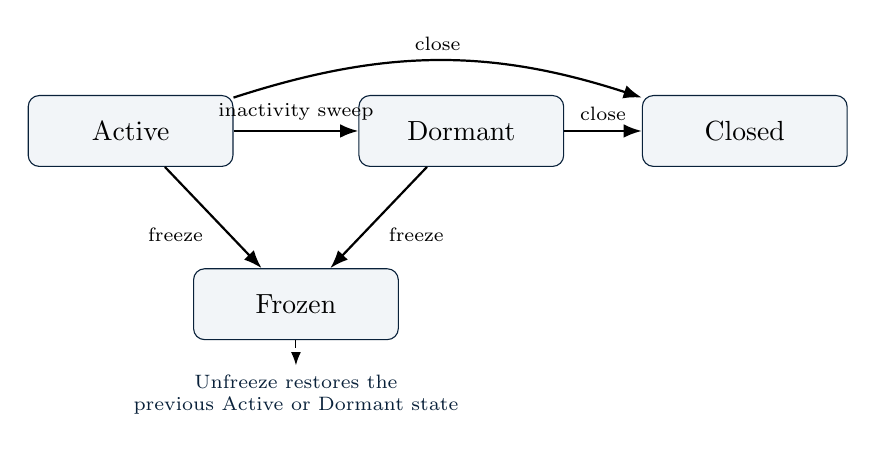
\begin{tikzpicture}[
  >=Latex,
  state/.style={draw=BankNavy,rounded corners,fill=SoftGray,minimum width=26mm,minimum height=9mm,align=center},
  note/.style={font=\scriptsize,align=center,text=BankNavy}
]
\node[state] (active) at (0,0) {Active};
\node[state] (dormant) at (4.2,0) {Dormant};
\node[state] (closed) at (7.8,0) {Closed};
\node[state] (frozen) at (2.1,-2.2) {Frozen};
\node[note] (restore) at (2.1,-3.35) {Unfreeze restores the\\previous Active or Dormant state};

\draw[->,thick] (active) -- node[above,font=\scriptsize]{inactivity sweep} (dormant);
\draw[->,thick] (active) -- node[below left,font=\scriptsize]{freeze} (frozen);
\draw[->,thick] (dormant) -- node[below right,font=\scriptsize]{freeze} (frozen);
\draw[->,thick] (active) to[bend left=18] node[above,font=\scriptsize]{close} (closed);
\draw[->,thick] (dormant) -- node[above,font=\scriptsize]{close} (closed);
\draw[dashed,->] (frozen) -- (restore);
\end{tikzpicture}
\caption{Account status transitions}
\end{figure}
Financial transactions require ownership. Withdrawal/transfer source accounts must be Active; deposits reject Closed/Frozen destinations; account closing is blocked for Frozen accounts and for accounts referenced by Pending transactions.

\section{Available balance and pending holds}
Posted \texttt{Account.Balance} is not the same as available balance. The helper view sums Pending outgoing transactions:
\[
\text{AvailableBalance}=\text{Balance}-\sum \text{PendingOutgoingAmount}.
\]
Minimum-balance checks use available balance so a customer cannot overspend by initiating multiple Pending withdrawals/transfers before finalization.

\section{Transaction amount-dependent delay}
\begin{center}
\begin{tabular}{rr}
\toprule\textbf{Amount} & \textbf{Completion delay}\\\midrule
$<5{,}000$ & 0 seconds\\
$<25{,}000$ & 60 seconds\\
$<100{,}000$ & 180 seconds\\
$\ge 100{,}000$ & 300 seconds\\
\bottomrule
\end{tabular}
\end{center}
\texttt{ReadyToCompleteAt} is therefore a scheduled processing time, not a random timestamp.

\section{Triggers}
\subsection{trg\_EMPB\_PreventDateOverlap}
\textbf{Table:} EMPB. Rejects overlapping branch-assignment date ranges for one employee.
\subsection{TR\_Account\_PreventCloseWithPending}
\textbf{Table:} Account. Rejects any transition to Closed while a Pending transaction references the account.
\subsection{TR\_Account\_SyncBranchLedger}
\textbf{Table:} Account. On balance insert/update, updates Branch.Balance and appends BranchLedger deltas.
\subsection{TR\_Customer\_PreventDeactivateWithPending}
\textbf{Table:} Customer. Rejects deactivation when any customer account has a Pending transaction.
\subsection{TR\_Transactions\_SyncInstallmentStatus}
\textbf{Table:} Transactions. When payment transaction completes/fails, synchronizes installment and loan status.
\subsection{TR\_Transactions\_EnforceTypePattern}
\textbf{Table:} Transactions. Enforces From/To account pattern for Deposit, Interest, Withdrawal, and Transfer.

\section{Effective-role function}
\texttt{dbo.fn\_UserHasEffectiveRole(UserID,RoleName)} does not merely check \texttt{UserRoles}. It requires an active user and active Customer profile. Employee requires an active linked employee. Admin additionally requires Employee role, active employee, \texttt{CanAccessAdmin=1}, and job title Branch Manager or Vice Manager. HighAdmin requires no linked EmployeeID and must not be combined with Employee/Admin.

\section{Transactional consistency and concurrency}
Critical procedures enable \texttt{SET XACT\_ABORT ON}, use \texttt{TRY/CATCH}, and wrap write operations in explicit transactions. Before rechecking balances or workflow state, they use locks such as \texttt{UPDLOCK} and \texttt{HOLDLOCK}. These measures reduce race conditions during balance updates, account-state changes, session logout, transfer approval, and manager replacement.

\chapter{Stored Procedures}
\section{Procedure design pattern}
Most write procedures follow this sequence:
\begin{enumerate}
\item Validate required inputs and enumerated values.
\item Resolve the caller and recalculate effective privilege.
\item Resolve ownership or current branch.
\item Begin an atomic transaction and lock target rows where necessary.
\item Recheck business state under lock.
\item Perform inserts\slash updates.
\item Insert an audit record.
\item Commit and return recordsets\slash output parameters; otherwise roll back and raise a structured SQL error.
\end{enumerate}

\section{Authentication and session}
\begingroup
\footnotesize
\setlength{\tabcolsep}{4pt}
\renewcommand{\arraystretch}{1.08}
\begin{longtable}{L{0.30\textwidth}L{0.22\textwidth}L{0.41\textwidth}}
\toprule\textbf{Procedure} & \textbf{Primary caller} & \textbf{Purpose and key rules}\\\midrule\endfirsthead
\toprule\textbf{Procedure} & \textbf{Primary caller} & \textbf{Purpose and key rules}\\\midrule\endhead
\nolinkurl{sp_User_SignUp} & Public & Creates\slash reuses a Customer through the customer procedure, creates Users row, hashes password, assigns Customer role, audits signup.\\
\nolinkurl{sp_User_Login} & Public & Validates one login identifier plus password, recalculates effective roles, creates a fixed-lifetime session token, returns identity\slash roles\slash ExpiresAt, audits login.\\
\nolinkurl{sp_User_ValidateSession} & Every protected request & Validates token, active state and expiry; recalculates effective Customer\slash Employee\slash Admin\slash HighAdmin roles and current branch; returns session context.\\
\nolinkurl{sp_User_Logout} & Authenticated & Marks the session inactive, writes LogoutTime, and audits logout.\\
\nolinkurl{sp_HighAdmin_CreateInitialUser} & One-time public setup & Creates the first HighAdmin only when none exists; links an active Customer identity, assigns Customer+HighAdmin, and audits creation.\\
\bottomrule
\end{longtable}
\endgroup
\section{Customer}
\begingroup
\footnotesize
\setlength{\tabcolsep}{4pt}
\renewcommand{\arraystretch}{1.08}
\begin{longtable}{L{0.30\textwidth}L{0.22\textwidth}L{0.41\textwidth}}
\toprule\textbf{Procedure} & \textbf{Primary caller} & \textbf{Purpose and key rules}\\\midrule\endfirsthead
\toprule\textbf{Procedure} & \textbf{Primary caller} & \textbf{Purpose and key rules}\\\midrule\endhead
\nolinkurl{sp_Customer_Create} & Employee\slash Admin\slash HighAdmin & Validates identity\slash contact uniqueness and age; inserts customer atomically and audits CustomerCreated.\\
\nolinkurl{sp_Customer_Search} & Employee\slash Admin\slash HighAdmin & Branch-scopes staff through customer-account relationships; HighAdmin sees all; supports name\slash NationalID\slash phone\slash email filters.\\
\nolinkurl{sp_Customer_GetByID} & Authenticated according to role & Returns own customer to Customer; current-branch customer to staff; any customer to HighAdmin.\\
\nolinkurl{sp_Customer_Update} & Customer self or scoped staff & Allows own profile or branch-scoped staff update; checks uniqueness and audits.\\
\nolinkurl{sp_Customer_Delete} & Scoped staff\slash HighAdmin & Soft-deactivates; blocks pending-transaction cases; branch scopes staff and audits.\\
\bottomrule
\end{longtable}
\endgroup
\section{Accounts}
\begingroup
\footnotesize
\setlength{\tabcolsep}{4pt}
\renewcommand{\arraystretch}{1.08}
\begin{longtable}{L{0.30\textwidth}L{0.22\textwidth}L{0.41\textwidth}}
\toprule\textbf{Procedure} & \textbf{Primary caller} & \textbf{Purpose and key rules}\\\midrule\endfirsthead
\toprule\textbf{Procedure} & \textbf{Primary caller} & \textbf{Purpose and key rules}\\\midrule\endhead
\nolinkurl{sp_AccountType_ListOptions} & Authenticated & Returns account-product options for controlled dropdowns.\\
\nolinkurl{sp_Account_Open} & Customer self-service & Generates 12-digit account number, validates branch\slash product\slash minimum deposit, inserts account and optional pending initial deposit, audits.\\
\nolinkurl{sp_Account_Search} & Authenticated & Customer own accounts; Employee\slash Admin current branch; HighAdmin all. Supports rich filters and calculates available balance.\\
\nolinkurl{sp_Account_GetInfo} & Authenticated & Returns account details under the same ownership\slash branch\slash all visibility model and audits view.\\
\nolinkurl{sp_Transaction_GetAccountHistory} & Authenticated & Returns newest transaction history for an authorized account and date range.\\
\nolinkurl{sp_Account_GetAvailableBalance} & Authenticated & Returns posted balance minus pending outgoing holds.\\
\nolinkurl{sp_Account_Freeze} & Employee\slash Admin\slash HighAdmin within scope & Stores previous Active\slash Dormant state and sets Frozen.\\
\nolinkurl{sp_Account_Unfreeze} & Admin\slash HighAdmin within scope & Restores FrozenPreviousStatus.\\
\nolinkurl{sp_Account_Close} & Employee\slash Admin\slash HighAdmin within scope & Blocks already closed, frozen, or pending-transaction accounts; sets close date and audits.\\
\nolinkurl{sp_Account_ChangeType} & Employee\slash Admin\slash HighAdmin within scope & Requires Active\slash Dormant, no pending transaction, sufficient available balance for target type; audits.\\
\nolinkurl{sp_Account_DormantSweep} & Admin\slash HighAdmin or job & Marks qualifying inactive accounts Dormant.\\
\nolinkurl{sp_Account_ApplyMonthlyInterest} & Admin\slash HighAdmin or job & Creates interest transactions for eligible account types atomically.\\
\bottomrule
\end{longtable}
\endgroup
\section{Transactions}
\begingroup
\footnotesize
\setlength{\tabcolsep}{4pt}
\renewcommand{\arraystretch}{1.08}
\begin{longtable}{L{0.30\textwidth}L{0.22\textwidth}L{0.41\textwidth}}
\toprule\textbf{Procedure} & \textbf{Primary caller} & \textbf{Purpose and key rules}\\\midrule\endfirsthead
\toprule\textbf{Procedure} & \textbf{Primary caller} & \textbf{Purpose and key rules}\\\midrule\endhead
\nolinkurl{sp_Transaction_Deposit} & Account owner & Validates destination ownership and account state; inserts Pending deposit with scheduled completion.\\
\nolinkurl{sp_Transaction_Withdrawal} & Account owner & Validates source ownership, Active state, minimum\slash available balance; inserts Pending withdrawal.\\
\nolinkurl{sp_Transaction_Transfer} & Source-account owner & Validates both accounts, ownership, status, available funds, and inserts Pending transfer.\\
\nolinkurl{sp_Transaction_Finalize} & Owner or system batch & Locks transaction\slash accounts, waits until ReadyToCompleteAt, posts balance changes, marks Completed\slash Failed, audits.\\
\nolinkurl{sp_Transaction_ProcessPendingBatch} & Admin\slash HighAdmin or SQL Agent & Set-based finalization of all ready Pending transactions.\\
\nolinkurl{sp_Transaction_Reverse} & Transaction owner & Cancels Pending or reverses Completed transaction while protecting minimum balance and linked installment semantics.\\
\bottomrule
\end{longtable}
\endgroup
\section{Loans and installments}
\begingroup
\footnotesize
\setlength{\tabcolsep}{4pt}
\renewcommand{\arraystretch}{1.08}
\begin{longtable}{L{0.30\textwidth}L{0.22\textwidth}L{0.41\textwidth}}
\toprule\textbf{Procedure} & \textbf{Primary caller} & \textbf{Purpose and key rules}\\\midrule\endfirsthead
\toprule\textbf{Procedure} & \textbf{Primary caller} & \textbf{Purpose and key rules}\\\midrule\endhead
\nolinkurl{sp_Loan_Create} & Employee\slash Admin\slash HighAdmin & Creates a branch loan and installment schedule atomically; validates active customer, branch, amount, rate, and installment count.\\
\nolinkurl{sp_Loan_GetStatus} & Authorized viewer & Returns loan summary plus installment recordset; customer ownership is enforced in SQL and staff scope is prevalidated by backend.\\
\nolinkurl{sp_Loan_PayInstallment} & Borrower only & Requires borrower-owned payment account, Active loan, unpaid\slash non-defaulted installment, and no existing pending payment; creates withdrawal transaction.\\
\nolinkurl{sp_Loan_ProcessOverdueInstallments} & Branch manager\slash Admin, HighAdmin, or job & Marks overdue installments Late\slash Defaulted and loans Defaulted according to branch scope; manual managers only current branch.\\
\bottomrule
\end{longtable}
\endgroup
\section{Branches, employees, and transfers}
\begingroup
\footnotesize
\setlength{\tabcolsep}{4pt}
\renewcommand{\arraystretch}{1.08}
\begin{longtable}{L{0.30\textwidth}L{0.22\textwidth}L{0.41\textwidth}}
\toprule\textbf{Procedure} & \textbf{Primary caller} & \textbf{Purpose and key rules}\\\midrule\endfirsthead
\toprule\textbf{Procedure} & \textbf{Primary caller} & \textbf{Purpose and key rules}\\\midrule\endhead
\nolinkurl{sp_Branch_ListOptions} & Authenticated & Returns non-sensitive BranchID\slash code\slash name\slash city for dropdowns.\\
\nolinkurl{sp_Branch_GetInfo} & Employee\slash Admin\slash HighAdmin & Normal employee sees current branch; managers current branch; HighAdmin all\slash selected.\\
\nolinkurl{sp_Employee_Hire} & Current-branch Admin & Creates ordinary employee and current EMPB assignment in manager branch; no login yet.\\
\nolinkurl{sp_Employee_CreateUserAccount} & Scoped Admin\slash HighAdmin & Creates\slash reuses customer identity and user, links employee, and assigns Customer+Employee.\\
\nolinkurl{sp_Employee_Search} & Employee\slash Admin\slash HighAdmin & Employee sees self; manager current branch; HighAdmin all\slash history.\\
\nolinkurl{sp_Employee_GetInfo} & Employee\slash Admin\slash HighAdmin & Same target visibility; returns employee and assignment details.\\
\nolinkurl{sp_EMPBranchHistory_Get} & Employee\slash Admin\slash HighAdmin & Self\slash current-branch\slash all history, with Vice Manager protection for Branch Manager records.\\
\nolinkurl{sp_Employee_ChangeJobTitle} & Scoped Admin\slash HighAdmin & Changes ordinary title; manager-level governance remains HighAdmin-specific.\\
\nolinkurl{sp_Employee_Suspend} & Scoped Admin\slash HighAdmin & Sets OnLeave and removes effective Employee\slash Admin privilege while preserving Customer access.\\
\nolinkurl{sp_Employee_Fire} & Scoped Admin\slash HighAdmin & Sets Terminated, closes current assignment, preserves customer login but removes effective staff privilege.\\
\nolinkurl{sp_EmployeeTransfer_RequestByEmployee} & Active Employee\slash Admin & Creates open transfer request to a different branch.\\
\nolinkurl{sp_EmployeeTransfer_RequestByManager} & Admin\slash HighAdmin & Creates transfer request for an eligible employee.\\
\nolinkurl{sp_EmployeeTransfer_ApproveCurrentManager} & Current-branch Admin & Approves\slash rejects first stage only for source branch.\\
\nolinkurl{sp_EmployeeTransfer_ApproveDestinationManager} & Destination Admin & Approves\slash rejects second stage; on approval closes old EMPB and creates new current assignment.\\
\bottomrule
\end{longtable}
\endgroup
\section{HighAdmin manager governance}
\begingroup
\footnotesize
\setlength{\tabcolsep}{4pt}
\renewcommand{\arraystretch}{1.08}
\begin{longtable}{L{0.30\textwidth}L{0.22\textwidth}L{0.41\textwidth}}
\toprule\textbf{Procedure} & \textbf{Primary caller} & \textbf{Purpose and key rules}\\\midrule\endfirsthead
\toprule\textbf{Procedure} & \textbf{Primary caller} & \textbf{Purpose and key rules}\\\midrule\endhead
\nolinkurl{sp_HighAdmin_HireManager} & HighAdmin & Requires existing BranchID and manager title; atomically creates\slash reuses Customer, Employee, EMPB, Users, and Customer+Employee+Admin roles.\\
\nolinkurl{sp_HighAdmin_PromoteToManager} & HighAdmin & Promotes active employee with login to Branch Manager\slash Vice Manager in target branch.\\
\nolinkurl{sp_HighAdmin_DowngradeManager} & HighAdmin & Changes manager to ordinary title and removes effective Admin capability.\\
\nolinkurl{sp_HighAdmin_SuspendManager} & HighAdmin & Suspends manager-level employee.\\
\nolinkurl{sp_HighAdmin_FireManager} & HighAdmin & Terminates manager-level employee.\\
\nolinkurl{sp_HighAdmin_ReplaceBranchManager} & HighAdmin & Atomically downgrades old manager, assigns\slash promotes replacement, and enforces one active Branch Manager.\\
\bottomrule
\end{longtable}
\endgroup

\section{Critical transaction flow}
\begin{figure}[H]
\centering
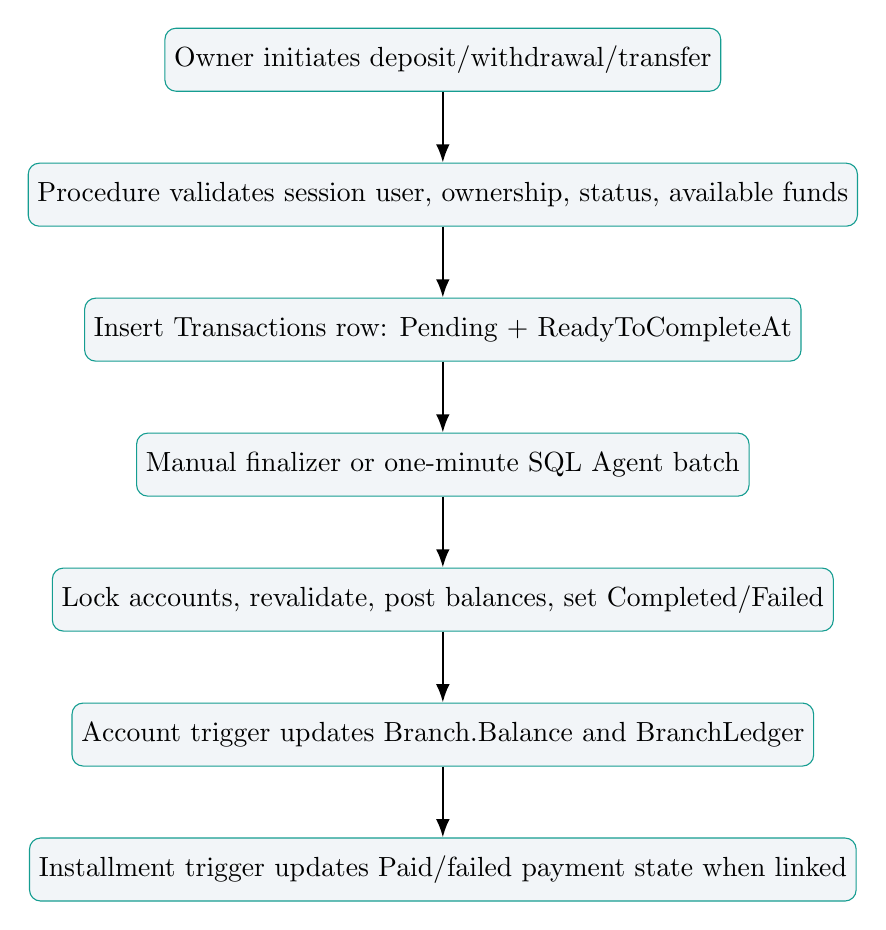
\begin{tikzpicture}[node distance=9mm,>=Latex,box/.style={draw=BankTeal,rounded corners,fill=SoftGray,minimum width=70mm,minimum height=8mm,align=center}]
\node[box] (a) {Owner initiates deposit\slash withdrawal\slash transfer};
\node[box,below=of a] (b) {Procedure validates session user, ownership, status, available funds};
\node[box,below=of b] (c) {Insert Transactions row: Pending + ReadyToCompleteAt};
\node[box,below=of c] (d) {Manual finalizer or one-minute SQL Agent batch};
\node[box,below=of d] (e) {Lock accounts, revalidate, post balances, set Completed\slash Failed};
\node[box,below=of e] (f) {Account trigger updates Branch.Balance and BranchLedger};
\node[box,below=of f] (g) {Installment trigger updates Paid\slash failed payment state when linked};
\draw[->,thick] (a)--(b);\draw[->,thick](b)--(c);\draw[->,thick](c)--(d);\draw[->,thick](d)--(e);\draw[->,thick](e)--(f);\draw[->,thick](f)--(g);
\end{tikzpicture}
\caption{Financial transaction lifecycle}
\end{figure}

\chapter{Views, Reports, and Scheduled Jobs}
\section{Reporting views}
\begin{longtable}{L{0.34\textwidth}L{0.60\textwidth}}
\toprule\textbf{View} & \textbf{Purpose}\\\midrule\endfirsthead
\toprule\textbf{View} & \textbf{Purpose}\\\midrule\endhead
\nolinkurl{vw_AccountPendingOutgoing} & Helper aggregate of Pending outgoing amounts by source account.\\
\nolinkurl{vw_CustomerBasicProfile} & Reporting-safe customer profile with masked NationalID and computed age.\\
\nolinkurl{vw_CustomerAccountSummary} & Customer/account/branch/type summary with posted, pending, and available balances.\\
\nolinkurl{vw_AccountOperationalSummary} & Operational account directory with masked customer ID and available balance.\\
\nolinkurl{vw_EmployeeDirectory} & Current employee directory; excludes salary and masks NationalID.\\
\nolinkurl{vw_HighAdmin_EmployeeBranchOverview} & Full current and historical employee/branch assignments including salary.\\
\nolinkurl{vw_PendingTransactions} & Pending transaction work queue.\\
\nolinkurl{vw_LoanOperationalSummary} & Loan summary with installment counts and remaining amount.\\
\nolinkurl{vw_HighAdmin_BranchFinancialOverview} & Branch aggregate reconciliation, account totals, and staffing counts.\\
\nolinkurl{vw_HighAdmin_UserAccessOverview} & User/customer/employee/role overview without password hashes or session tokens.\\
\nolinkurl{vw_AuditTrail_Safe} & Audit records joined to username.\\
\nolinkurl{vw_BranchLedgerReport} & Branch ledger joined to branch identity.\\
\nolinkurl{vw_DailyTransactionSummary} & Daily counts and amounts by type and status.\\
\nolinkurl{vw_AccountStatusSummary} & Account counts and balances by branch/status.\\
\nolinkurl{vw_LoanOverdueSummary} & Overdue count, amount, and oldest due date by loan.\\
\bottomrule
\end{longtable}

\section{API report catalogue}
{\footnotesize
\setlength{\tabcolsep}{4pt}
\renewcommand{\arraystretch}{1.10}
\begin{longtable}{L{0.27\textwidth}L{0.45\textwidth}L{0.20\textwidth}}
\toprule\textbf{Report key} & \textbf{Authorized roles and data scope} & \textbf{Default order}\\\midrule\endfirsthead
\toprule\textbf{Report key} & \textbf{Authorized roles and data scope} & \textbf{Default order}\\\midrule\endhead
\nolinkurl{customer-basic-profile} & Employee\slash Admin\slash HighAdmin; staff see customers related to the current branch through account ownership. & RegistrationDate DESC\\
\nolinkurl{customer-account-summary} & Employee\slash Admin\slash HighAdmin; current branch for staff. & OpenDate DESC\\
\nolinkurl{account-operational-summary} & Employee\slash Admin\slash HighAdmin; current branch for staff. & OpenDate DESC\\
\nolinkurl{employee-directory} & Employee\slash Admin\slash HighAdmin; self or current branch for staff according to role. & HireDate DESC\\
\nolinkurl{pending-transactions} & Employee\slash Admin\slash HighAdmin; accounts linked to the current branch for staff. & TransactionDate DESC\\
\nolinkurl{loan-operational-summary} & Employee\slash Admin\slash HighAdmin; current branch for staff. & StartDate DESC\\
\nolinkurl{daily-transaction-summary} & Admin\slash HighAdmin; role-protected aggregate. & TransactionDay DESC\\
\nolinkurl{account-status-summary} & Admin\slash HighAdmin; current branch for Admin, all for HighAdmin. & BranchID DESC\\
\nolinkurl{loan-overdue-summary} & Admin\slash HighAdmin; current branch for Admin, all for HighAdmin. & Oldest overdue date DESC\\
\texttt{highadmin-employee-}\newline\texttt{branch-overview} & HighAdmin only; all current and historical assignments. & StartDate DESC\\
\texttt{highadmin-branch-}\newline\texttt{financial-overview} & HighAdmin only; all branches. & BranchID DESC\\
\texttt{highadmin-user-access-}\newline\texttt{overview} & HighAdmin only; all application users and effective access context. & UserID DESC\\
\nolinkurl{audit-trail} & HighAdmin only; all rows through the audit SQL pool. & ActionDate DESC\\
\nolinkurl{branch-ledger} & HighAdmin only; all rows through the audit SQL pool. & EntryDate DESC\\
\bottomrule
\end{longtable}
}
The backend chooses the view name and ORDER BY expression from a hard-coded map. The client cannot submit a view name or SQL identifier. Only paging and branch values are parameters. This is why the small dynamic report query remains safe from SQL injection.

\section{Database pools and least privilege}
The backend has four connection pools:
\begin{itemize}
\item \textbf{app}: normal procedure execution and limited operational views.
\item \textbf{report}: ordinary reporting views.
\item \textbf{audit}: audit trail and branch ledger views.
\item \textbf{highadminReport}: HighAdmin-only reporting views.
\end{itemize}
SQL Server database roles are \texttt{dbrole\_bank\_app\_executor}, \texttt{dbrole\_bank\_reporting}, \texttt{dbrole\_bank\_auditor}, \texttt{dbrole\_bank\_highadmin\_viewer}, and \texttt{dbrole\_bank\_maintenance}. Direct DML permissions on base tables are revoked from application/report personas; access is through procedure execution and selected views.

\section{SQL Server Agent jobs}
{\footnotesize
\setlength{\tabcolsep}{4pt}
\renewcommand{\arraystretch}{1.12}
\begin{longtable}{L{0.27\textwidth}L{0.31\textwidth}L{0.33\textwidth}}
\toprule\textbf{Job and schedule} & \textbf{Command} & \textbf{Purpose}\\\midrule\endfirsthead
\toprule\textbf{Job and schedule} & \textbf{Command} & \textbf{Purpose}\\\midrule\endhead
\textbf{Process Pending Bank Transactions}\newline Every minute & \texttt{EXEC }\nolinkurl{dbo.sp_Transaction_ProcessPendingBatch;} & Completes all Pending transactions whose ReadyToCompleteAt has arrived.\\
\textbf{Process Overdue Loan Installments}\newline Daily at 00:00 & \texttt{EXEC }\nolinkurl{dbo.sp_Loan_ProcessOverdueInstallments;} & Marks late/defaulted installments and related loans across all branches.\\
\textbf{Apply Monthly Account Interest}\newline Monthly, day 1 at 00:05 & \texttt{EXEC }\nolinkurl{dbo.sp_Account_ApplyMonthlyInterest;} & Creates eligible interest-credit transactions.\\
\bottomrule
\end{longtable}
}

\chapter{Authentication, Authorization, Sessions, and Audit}
\section{Login and session sequence}
\begin{figure}[H]
\centering
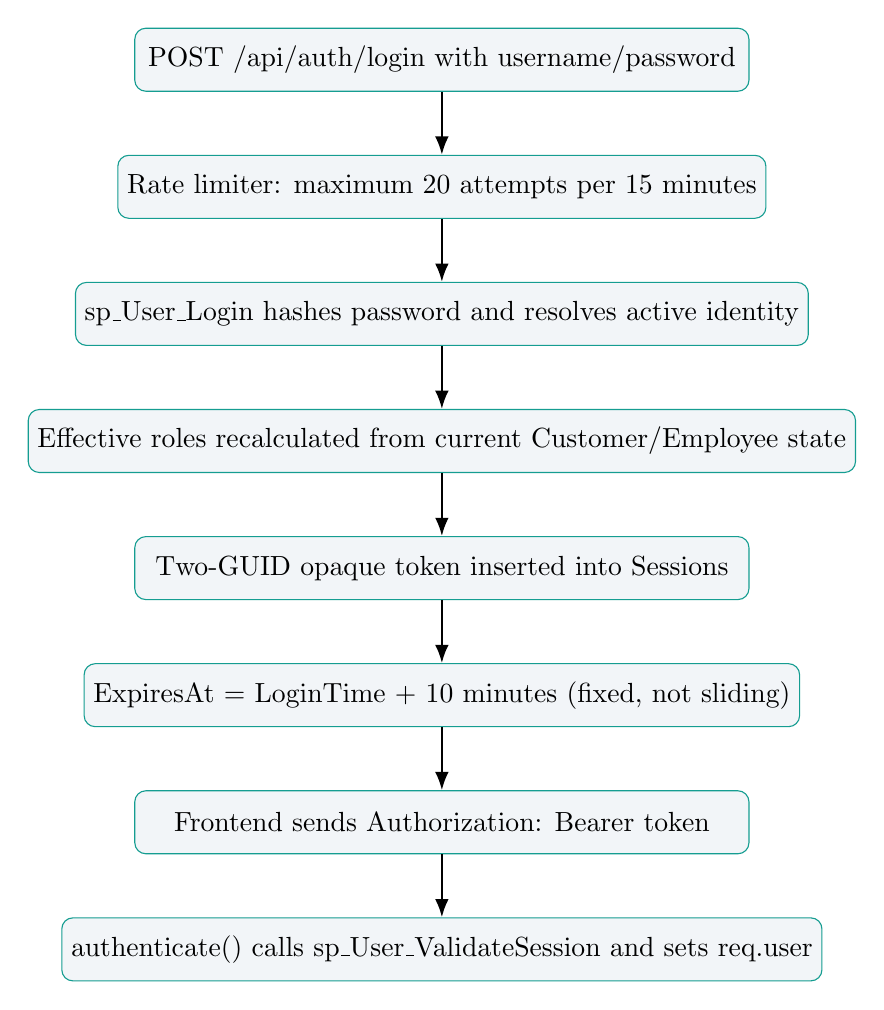
\begin{tikzpicture}[node distance=8mm,>=Latex,box/.style={draw=BankTeal,rounded corners,fill=SoftGray,minimum width=78mm,minimum height=8mm,align=center}]
\node[box] (a) {POST /api/auth/login with username/password};
\node[box,below=of a] (b) {Rate limiter: maximum 20 attempts per 15 minutes};
\node[box,below=of b] (c) {sp\_User\_Login hashes password and resolves active identity};
\node[box,below=of c] (d) {Effective roles recalculated from current Customer/Employee state};
\node[box,below=of d] (e) {Two-GUID opaque token inserted into Sessions};
\node[box,below=of e] (f) {ExpiresAt = LoginTime + 10 minutes (fixed, not sliding)};
\node[box,below=of f] (g) {Frontend sends Authorization: Bearer token};
\node[box,below=of g] (h) {authenticate() calls sp\_User\_ValidateSession and sets req.user};
\draw[->,thick](a)--(b);\draw[->,thick](b)--(c);\draw[->,thick](c)--(d);\draw[->,thick](d)--(e);\draw[->,thick](e)--(f);\draw[->,thick](f)--(g);\draw[->,thick](g)--(h);
\end{tikzpicture}
\caption{Authentication and session validation}
\end{figure}

\section{How req.user is created}
\begin{lstlisting}[language=JavaScript,caption={Authentication middleware concept}]
const token = extractBearerToken(req);
const result = await executeProcedure('dbo.sp_User_ValidateSession', {
  inputs: { SessionToken: TYPES.token, RequiredRole: TYPES.string50 },
  values: { SessionToken: token, RequiredRole: requiredRole }
});
const user = result.recordset[0];
req.sessionToken = token;
req.user = { ...user, roles: parseRoles(user.EffectiveRoles) };
next();
\end{lstlisting}
\texttt{req.user.UserID} is therefore a custom Express request property populated from a validated SQL result. It is not supplied by the browser and is unrelated to ORM behavior.

\section{Assigned roles versus effective roles}
\begin{longtable}{L{0.18\textwidth}L{0.73\textwidth}}
\toprule\textbf{Role} & \textbf{Effective-role conditions}\\\midrule
Customer & Active Users row, active linked Customer, and assigned Customer role.\\
Employee & Customer conditions plus linked Employee, assigned Employee role, and Employee.EmpStatus=Active.\\
Admin & Effective Employee plus assigned Admin role, CanAccessAdmin=1, and title Branch Manager or Vice Manager.\\
HighAdmin & Active Customer identity, assigned HighAdmin, no EmployeeID, and no Employee/Admin role combination.\\
\bottomrule
\end{longtable}
This design means OnLeave/Terminated staff can retain personal Customer access while losing employee/admin privilege immediately, even with an existing token.

\section{Branch and ownership authorization}
\begin{itemize}
\item Customer and \texttt{scope=mine}: CustomerID from validated session.
\item Employee/Admin operational scope: CurrentBranchID from the current \texttt{EMPB} assignment.
\item HighAdmin operational scope: all branches unless a branch is explicitly selected for a supported operation.
\item Transactions: owner-only regardless of Employee/Admin/HighAdmin roles.
\item Installment payment: borrower-only, and the payment account must belong to the same borrower.
\item Managers: employees and customers only from their current branch; customer-to-branch relation is derived through Account.
\end{itemize}

\section{Auditing}
Audit entries are inserted by procedures for login, logout, expiry, signup, searches, views, customer/account/transaction/loan/employee/manager operations, transfers, and maintenance. HighAdmin reads \texttt{vw\_AuditTrail\_Safe}; raw password hashes and session tokens are not exposed by reporting views. Branch balance changes are separately represented in \texttt{BranchLedger}.

\chapter{SQL Injection Control and Direct SQL Data Access}
\section{Evidence that the project does not use an ORM}
The backend accesses SQL Server directly through the \texttt{mssql} package. In this project, \texttt{mssql} is used as a database driver: it opens SQL Server connection pools, binds typed parameters, executes named stored procedures or controlled queries, and returns recordsets. It does not map database tables to JavaScript classes.

The conclusion that no ORM is used is supported by the repository itself:

\begin{longtable}{L{0.28\textwidth}L{0.65\textwidth}}
\toprule
\textbf{Evidence} & \textbf{What is present in this project}\\
\midrule\endfirsthead
\toprule\textbf{Evidence} & \textbf{What is present in this project}\\\midrule\endhead
Dependencies & \texttt{package.json} contains \texttt{mssql}, Express, CORS, Helmet, Morgan, rate limiting, and environment support. It does not contain Sequelize, TypeORM, Prisma, Knex, Objection, Bookshelf, MikroORM, or Drizzle.\\
Database connection & \codepath{src/config/db.js} imports \texttt{mssql} and creates \texttt{sql.ConnectionPool} objects directly.\\
Data-access helper & \codepath{src/utils/procedure.js} calls \texttt{request.input(...)} and then \texttt{request.execute(procedureName)} or \texttt{request.query(queryText)}.\\
Routes & Route files name the SQL procedure explicitly and define each SQL type explicitly. For example, the account-opening route calls \texttt{dbo.sp\_Account\_Open} and binds \texttt{UserID}, \texttt{BranchID}, \texttt{AccountTypeID}, and \texttt{InitialDeposit}.\\
Project structure & There is no ORM model or entity layer, no \texttt{schema.prisma}, no generated migration folder, and no repository pattern built on ORM entities.\\
Business logic & Balance checks, account ownership, loan rules, branch scope, audit insertion, locks, transactions, and state transitions are implemented in T-SQL procedures, triggers, constraints, and functions.\\
Returned data & The backend reads SQL \texttt{recordset}, \texttt{recordsets}, output parameters, and \texttt{rowsAffected}; it does not receive mapped entity instances.\\
\bottomrule
\end{longtable}

\begin{lstlisting}[language=JavaScript,caption={Direct SQL Server connection pool from \texttt{src/config/db.js}}]
const sql = require('mssql');

const pool = new sql.ConnectionPool(config);
pools.set(name, pool.connect());
\end{lstlisting}

\begin{lstlisting}[language=JavaScript,caption={Typed procedure execution from \texttt{src/utils/procedure.js}}]
const pool = await getPool(poolName);
const request = pool.request();

request.input('UserID', sql.Int, values.UserID);
request.input('BranchID', sql.Int, values.BranchID);

const result = await request.execute('dbo.sp_Account_Open');
\end{lstlisting}

\begin{defensebox}[Repository check]
Open \texttt{package.json}, \codepath{src/config/db.js}, \codepath{src/utils/procedure.js}, and one route file. The dependency list shows no ORM package; the source code shows a direct \texttt{mssql} connection, explicit SQL types, and explicit stored-procedure names. The corresponding T-SQL procedure shows where the business rules are implemented.
\end{defensebox}

\section{Difference between a driver and an ORM}
A SQL driver provides a communication layer between the application and the database. An ORM adds an object model above that layer and normally maps tables to classes, creates queries from method calls, tracks entity changes, and manages relationships through model definitions. None of those ORM services is used here. The application sends parameters to SQL Server and relies on database objects written manually.

\section{SQL injection controls}
\begin{enumerate}
\item User-supplied values are passed with explicit SQL types through \texttt{request.input}.
\item Stored procedures receive values as parameters; user text is not concatenated into SQL statements.
\item Report queries use view names and ordering expressions selected from a server-owned whitelist.
\item Paging values, branch identifiers, record identifiers, names, dates, amounts, and statuses remain bound parameters.
\item Route validation and SQL-side validation provide two separate checks.
\item Database roles restrict direct access to base tables and grant only the required procedures or views.
\end{enumerate}

\begin{warningbox}[Important distinction]
Stored procedures are not automatically immune to SQL injection. They are safe only when values remain parameters or when any dynamic identifier is selected from trusted server code. In this project, client input is never used as an arbitrary table name, view name, column name, or SQL fragment.
\end{warningbox}

\chapter{Backend Architecture}
\section{Technology and startup}
The backend uses Node.js and Express. Supporting packages provide SQL Server access, environment configuration, security headers, CORS, request logging, and rate limiting. \codepath{src/server.js} starts the HTTP listener and closes the SQL pools during shutdown. \codepath{src/app.js} installs the middleware, health route, module routers, 404 handler, and centralized error handler.

\section{Configuration and database connection}
\texttt{src/config/env.js} validates environment variables and supplies defaults. \texttt{src/config/db.js} lazily creates named connection pools. SQL dates use \texttt{DB\_USE\_UTC=false} so SQL Server local \texttt{DATETIME} values are not incorrectly interpreted as UTC. Pooling avoids opening a new database connection for every request.

\section{Request handling pattern}
\begin{enumerate}
\item Express matches the route and parses JSON/query/path parameters.
\item \texttt{authenticate()} validates the bearer session for protected routes.
\item \texttt{authorize(...roles)} performs broad application-role checks.
\item Route code overrides identity/branch fields with trusted \texttt{req.user} values.
\item \texttt{executeProcedure} or \texttt{executeQuery} binds typed parameters and selects the correct pool.
\item SQL Server performs detailed authorization, transaction, audit, and integrity logic.
\item \texttt{ok}/\texttt{created} normalizes DATE vs DATETIME values and returns a consistent JSON envelope.
\item SQL errors are normalized into structured HTTP errors; unknown routes return 404.
\end{enumerate}

\section{API response shape}
\begin{lstlisting}[language=JavaScript]
{
  "success": true,
  "data": [...],
  "meta": {
    "accessScope": "branch",
    "branchID": 2,
    "dateFields": { "TransactionDate": "datetime" }
  }
}
\end{lstlisting}
Failures use \texttt{success:false} and \texttt{error.message}; SQL errors also expose number/state/procedure/line in development.

\section{Complete API inventory}
The following tables list the implemented HTTP surface. Endpoint paths and SQL object names are typeset with breakable monospaced text so that the inventory remains readable in print.

{\footnotesize
\setlength{\tabcolsep}{4pt}
\renewcommand{\arraystretch}{1.12}

\subsection{Setup, authentication, and customers}
\begin{longtable}{L{0.40\textwidth}L{0.27\textwidth}L{0.24\textwidth}}
\toprule\textbf{Method and endpoint} & \textbf{Access} & \textbf{SQL target}\\\midrule\endfirsthead
\toprule\textbf{Method and endpoint} & \textbf{Access} & \textbf{SQL target}\\\midrule\endhead
POST \nolinkurl{/api/setup/initial-high-admin} & Public, one-time & \nolinkurl{sp_HighAdmin_CreateInitialUser}\\
POST \nolinkurl{/api/auth/signup} & Public & \nolinkurl{sp_User_SignUp}\\
POST \nolinkurl{/api/auth/login} & Public, rate-limited & \nolinkurl{sp_User_Login}\\
POST \nolinkurl{/api/auth/logout} & Authenticated & \nolinkurl{sp_User_Logout}\\
GET \nolinkurl{/api/auth/me} & Authenticated & Validated session context\\
GET \nolinkurl{/api/customers} & Employee/Admin: current branch; HighAdmin: all & \nolinkurl{sp_Customer_Search}\\
POST \nolinkurl{/api/customers} & Employee/Admin/HighAdmin & \nolinkurl{sp_Customer_Create}\\
PUT \nolinkurl{/api/customers/:customerID} & Branch-scoped staff or HighAdmin & \nolinkurl{sp_Customer_Update}\\
DELETE \nolinkurl{/api/customers/:customerID} & Branch-scoped staff or HighAdmin & \nolinkurl{sp_Customer_Delete}\\
\bottomrule
\end{longtable}

\subsection{Accounts and transactions}
\begin{longtable}{L{0.40\textwidth}L{0.27\textwidth}L{0.24\textwidth}}
\toprule\textbf{Method and endpoint} & \textbf{Access} & \textbf{SQL target}\\\midrule\endfirsthead
\toprule\textbf{Method and endpoint} & \textbf{Access} & \textbf{SQL target}\\\midrule\endhead
GET \nolinkurl{/api/accounts/mine} & Authenticated user's own accounts & \nolinkurl{sp_Account_Search}\\
GET \nolinkurl{/api/accounts} & Customer: own; Employee/Admin: branch; HighAdmin: all & \nolinkurl{sp_Account_Search}\\
GET \nolinkurl{/api/accounts/options/account-types} & Authenticated safe catalogue & \nolinkurl{sp_AccountType_ListOptions}\\
GET \nolinkurl{/api/accounts/:accountID} & Authorized owner/branch/all viewer & \nolinkurl{sp_Account_GetInfo}\\
GET \nolinkurl{/api/accounts/:accountID/history} & Authorized owner/branch/all viewer & \nolinkurl{sp_Transaction_GetAccountHistory}\\
POST \nolinkurl{/api/accounts} & Customer self-service & \nolinkurl{sp_Account_Open}\\
POST \nolinkurl{/api/accounts/:id/freeze} & Scoped Employee/Admin/HighAdmin & \nolinkurl{sp_Account_Freeze}\\
POST \nolinkurl{/api/accounts/:id/unfreeze} & Scoped Admin/HighAdmin & \nolinkurl{sp_Account_Unfreeze}\\
POST \nolinkurl{/api/accounts/:id/close} & Scoped Employee/Admin/HighAdmin & \nolinkurl{sp_Account_Close}\\
POST \nolinkurl{/api/accounts/:id/change-type} & Scoped Employee/Admin/HighAdmin & \nolinkurl{sp_Account_ChangeType}\\
POST \nolinkurl{/api/transactions/deposit} & Account owner only & \nolinkurl{sp_Transaction_Deposit}\\
POST \nolinkurl{/api/transactions/withdraw} & Account owner only & \nolinkurl{sp_Transaction_Withdrawal}\\
POST \nolinkurl{/api/transactions/transfer} & Source-account owner only & \nolinkurl{sp_Transaction_Transfer}\\
POST \nolinkurl{/api/transactions/:id/finalize} & Transaction/account owner policy & \nolinkurl{sp_Transaction_Finalize}\\
POST \nolinkurl{/api/transactions/:id/reverse} & Transaction/account owner policy & \nolinkurl{sp_Transaction_Reverse}\\
POST \nolinkurl{/api/transactions/maintenance/process-pending-batch} & Admin/HighAdmin maintenance & \nolinkurl{sp_Transaction_ProcessPendingBatch}\\
\bottomrule
\end{longtable}

\subsection{Loans, employees, and transfers}
\begin{longtable}{L{0.40\textwidth}L{0.27\textwidth}L{0.24\textwidth}}
\toprule\textbf{Method and endpoint} & \textbf{Access} & \textbf{SQL target}\\\midrule\endfirsthead
\toprule\textbf{Method and endpoint} & \textbf{Access} & \textbf{SQL target}\\\midrule\endhead
GET \nolinkurl{/api/loans} & Customer: own; Employee/Admin: branch; HighAdmin: all & \nolinkurl{vw_LoanOperationalSummary}\\
POST \nolinkurl{/api/loans} & Employee/Admin current branch; HighAdmin any branch & \nolinkurl{sp_Loan_Create}\\
GET \nolinkurl{/api/loans/:id/status} & Authorized owner/branch/all viewer & \nolinkurl{sp_Loan_GetStatus}\\
POST \nolinkurl{/api/loans/installments/:id/pay} & Borrower only, using an owned payment account & \nolinkurl{sp_Loan_PayInstallment}\\
POST \nolinkurl{/api/loans/maintenance/process-overdue-installments} & Admin current branch; HighAdmin all or selected branch & \nolinkurl{sp_Loan_ProcessOverdueInstallments}\\
GET \nolinkurl{/api/employees} & Employee: self; Admin: branch; HighAdmin: all & \nolinkurl{sp_Employee_Search}\\
GET \nolinkurl{/api/employees/:id} & Employee: self; Admin: branch; HighAdmin: all & \nolinkurl{sp_Employee_GetInfo}\\
POST \nolinkurl{/api/employees} & Admin's current branch, ordinary job title & \nolinkurl{sp_Employee_Hire}\\
POST \nolinkurl{/api/employees/:id/create-user-account} & Scoped Admin/HighAdmin & \nolinkurl{sp_Employee_CreateUserAccount}\\
POST \nolinkurl{/api/employees/:id/change-job-title} & Scoped Admin/HighAdmin & \nolinkurl{sp_Employee_ChangeJobTitle}\\
POST \nolinkurl{/api/employees/:id/suspend} & Scoped Admin/HighAdmin & \nolinkurl{sp_Employee_Suspend}\\
POST \nolinkurl{/api/employees/:id/fire} & Scoped Admin/HighAdmin & \nolinkurl{sp_Employee_Fire}\\
GET \nolinkurl{/api/employees/:id/branch-history} & Employee: self; Admin: branch; HighAdmin: all & \nolinkurl{sp_EMPBranchHistory_Get}\\
POST \nolinkurl{/api/employee-transfers/request-by-employee} & Employee/Admin & \nolinkurl{sp_EmployeeTransfer_RequestByEmployee}\\
POST \nolinkurl{/api/employee-transfers/request-by-manager} & Admin/HighAdmin & \nolinkurl{sp_EmployeeTransfer_RequestByManager}\\
POST \nolinkurl{/api/employee-transfers/:id/current-manager-decision} & Admin of source branch & \nolinkurl{sp_EmployeeTransfer_ApproveCurrentManager}\\
POST \nolinkurl{/api/employee-transfers/:id/destination-manager-decision} & Admin of destination branch & \nolinkurl{sp_EmployeeTransfer_ApproveDestinationManager}\\
\bottomrule
\end{longtable}

\subsection{Branches, HighAdmin governance, and reports}
\begin{longtable}{L{0.40\textwidth}L{0.27\textwidth}L{0.24\textwidth}}
\toprule\textbf{Method and endpoint} & \textbf{Access} & \textbf{SQL target}\\\midrule\endfirsthead
\toprule\textbf{Method and endpoint} & \textbf{Access} & \textbf{SQL target}\\\midrule\endhead
GET \nolinkurl{/api/branches/options} & Authenticated safe catalogue & \nolinkurl{sp_Branch_ListOptions}\\
GET \nolinkurl{/api/branches} & Employee/Admin/HighAdmin & \nolinkurl{sp_Branch_GetInfo}\\
POST \nolinkurl{/api/highadmin/managers} & HighAdmin; branch ID mandatory & \nolinkurl{sp_HighAdmin_HireManager}\\
POST \nolinkurl{/api/highadmin/managers/:id/promote} & HighAdmin & \nolinkurl{sp_HighAdmin_PromoteToManager}\\
POST \nolinkurl{/api/highadmin/managers/:id/downgrade} & HighAdmin & \nolinkurl{sp_HighAdmin_DowngradeManager}\\
POST \nolinkurl{/api/highadmin/managers/:id/suspend} & HighAdmin & \nolinkurl{sp_HighAdmin_SuspendManager}\\
POST \nolinkurl{/api/highadmin/managers/:id/fire} & HighAdmin & \nolinkurl{sp_HighAdmin_FireManager}\\
POST \nolinkurl{/api/highadmin/branches/:id/replace-manager} & HighAdmin & \nolinkurl{sp_HighAdmin_ReplaceBranchManager}\\
GET \nolinkurl{/api/reports} & Authenticated report catalogue & Server-side report map\\
GET \nolinkurl{/api/reports/:reportKey} & Role- and branch-scoped & Server-whitelisted SELECT from a protected view\\
\bottomrule
\end{longtable}
}


\chapter{Frontend Architecture}
\section{Technology and file organization}
The frontend intentionally uses vanilla HTML, CSS, and JavaScript. A dependency-free Node static server serves the files. Main pages are \texttt{index.html}, \texttt{customer.html}, \texttt{employee.html}, \texttt{admin.html}, and \texttt{highadmin.html}. Shared behavior is divided into:
\begin{itemize}
\item \texttt{config.js}: backend base URL, storage keys, role hierarchy, role-to-page routing.
\item \texttt{session.js}: token/user persistence, role normalization, fixed-expiry timer, preview mode.
\item \texttt{api.js}: \texttt{fetch}, Authorization header, timeout, JSON conversion, network/401 handling.
\item \texttt{workspace.js}: sidebar, active section, content lifecycle, current user, responsive workspace shell.
\item \texttt{features.js}: forms, tables, report viewers, actions, branch overview, account/loan/customer/employee modules.
\item \texttt{ui.js}: modals, toasts, tables, date/currency formatting, CSV export, safe rendering helpers.
\item role page scripts: define navigation and map section IDs to shared feature implementations.
\end{itemize}

\section{Authentication page}
The authentication page contains Sign in, Customer signup, connection settings, first HighAdmin setup, and preview mode. The left visual panel keeps only the BankManagement logo over the background image. Connection settings update the backend URL in local storage and test \texttt{/api/health}.

\section{Frontend session behavior}
The token and user object are stored in \texttt{sessionStorage} or \texttt{localStorage} depending on the persistence checkbox. The API wrapper adds \texttt{Authorization: Bearer <token>}. A local timer redirects after \texttt{ExpiresAt}, but the backend/SQL validation remains authoritative. A manipulated browser clock or disabled JavaScript cannot extend the server session.

\section{Role-aware workspaces}
\begin{longtable}{L{0.16\textwidth}L{0.76\textwidth}}
\toprule\textbf{Workspace} & \textbf{Key sections}\\\midrule
Customer & Overview, personal accounts, transactions, personal loans/installments, profile/security.\\
Employee & Current branch overview, branch customers/accounts/loans read/manage scope, own accounts/transactions/loans, own employee record, transfer request, operational reports.\\
Admin & Current branch overview, branch customers/accounts/loans, overdue processing, branch employee actions, transfer approvals, reports, maintenance, own portfolio.\\
HighAdmin & Enterprise overview, manager governance, all customers/accounts/loans/employees/branches, all reports, audit/ledger, maintenance, own portfolio.\\
\bottomrule
\end{longtable}

\section{Dynamic dropdowns and branch overview}
Branch and account-type choices use safe catalogue endpoints rather than free numeric text where possible. Other forms dynamically load allowed accounts, customers, employees, destination branches, and managers. Employee/Admin home pages use the CurrentBranchID from the validated session and display branch details and operational totals; the user cannot choose a different branch for that dashboard.

\section{Date handling}
The backend sends SQL DATE values as \texttt{YYYY-MM-DD} to avoid timezone day shifts, and DATETIME values as ISO instants. Metadata identifies date fields. The frontend uses the browser locale for readable display and the same formatter for tables, details, audit text, history, and CSV exports.

\chapter{End-to-End Use Cases}
\section{Customer opens an account}
\begin{enumerate}
\item Frontend loads safe branch and account-type dropdowns.
\item Customer submits branchID, accountTypeID, and optional initial deposit.
\item Route replaces UserID with \texttt{req.user.UserID}.
\item \texttt{sp\_Account\_Open} resolves the linked active Customer, generates account number, validates product/branch/minimum, inserts account.
\item If deposit is supplied, it invokes the deposit procedure and returns a Pending transaction and ready time.
\item Audit records capture opening; finalization later posts the initial deposit.
\end{enumerate}

\section{Manager views and acts on branch accounts}
The manager's token resolves CurrentBranchID. \texttt{GET /api/accounts} forces that branch. Lifecycle actions first assert visibility, then SQL procedures revalidate effective privilege and account state. The manager may freeze, unfreeze, change type, or close according to role/state, but cannot deposit, withdraw, transfer, finalize, reverse, or pay installments unless personally owning the relevant account/loan.

\section{Employee hiring}
A branch Admin uses \texttt{sp\_Employee\_Hire}; the procedure derives the manager's branch and creates Employee+EMPB only. A separate login-creation operation creates/reuses the Customer identity, creates Users, links Employee, and assigns Customer+Employee. HighAdmin manager hiring instead requires an explicit existing BranchID and atomically creates/reuses Customer, creates Employee+EMPB+Users, and assigns Customer+Employee+Admin.

\section{Loan installment payment}
The route verifies the payment account is in the caller's personal portfolio. SQL resolves installment $\rightarrow$ loan $\rightarrow$ borrower and rejects non-borrowers. It creates a Pending withdrawal transaction and stores the transaction ID in the installment. On completion, the synchronization trigger marks the installment Paid and may mark the loan Paid.

\chapter{Installation, Operation, and Demonstration}
\section{Database installation order}
\begin{enumerate}
\item Create database and SQL logins.
\item Run the full table-creation script on a clean database, or apply the numbered migration installers to an existing database.
\item Install password hash function, schema-support scripts, access rules, effective-role function, triggers, procedures, reporting/security views, database users/roles, and optional Agent jobs.
\item Load realistic sample data only after all objects are installed.
\end{enumerate}

\section{Run commands}
\begin{lstlisting}[language=Bash]
# Backend
npm install
npm run dev

# Frontend (separate terminal)
npm start
\end{lstlisting}
Default URLs are \texttt{http://127.0.0.1:4000} and \texttt{http://127.0.0.1:5500}. The backend \texttt{.env} contains SQL credentials, CORS origins, separate report credentials, \texttt{DB\_USE\_UTC=false}, and \texttt{SESSION\_TTL\_MINUTES=10}.

\section{Recommended live defense demonstration}
\begin{enumerate}
\item Show the ER diagrams and one table definition with PK/FK/CHECK constraints.
\item Login as Customer and show own accounts; attempt another customer's account and show rejection.
\item Initiate a transaction; show Pending row, ReadyToCompleteAt, available-balance hold, then finalize/process batch.
\item Login as branch manager; show current branch overview, branch-only employees/customers/accounts/loans, and account lifecycle action without transaction permission.
\item Pay an installment as borrower; show trigger-updated installment state after transaction completion.
\item Process overdue installments as manager and explain current-branch restriction.
\item Login as HighAdmin; show all reports, safe audit, branch ledger, and manager hiring with mandatory branch dropdown.
\item In code, show \texttt{request.input}, \texttt{authenticate()}, and one stored procedure with transaction/locks/audit.
\end{enumerate}

\chapter{Testing and Verification}
The Postman collection covers health, sample logins, identity resolution, effective role states, read-only fixtures, authorization boundaries, eight intentional SQL error scenarios, all fourteen reports, and optional write workflows. The latest recorded full run before the final UI-oriented patches completed 108 requests with 457 passing assertions and 9 failures. The remaining failures were concentrated in mutable optional workflows (previously transferred employee and a pending transaction before account-type change), rather than broad authentication, reports, or error-injection failures. For a final defense run, reseed/reset sample data or run stable folders separately from state-changing workflows.

\section{Recommended additional tests}
\begin{itemize}
\item Expired token exactly after ten minutes and explicit logout revocation.
\item Parallel withdrawals/transfers to demonstrate pending holds and locks.
\item Manager attempts cross-branch employee/customer/account/loan access.
\item HighAdmin manager hire with missing/invalid branchID.
\item Customer attempts staff report and manager attempts HighAdmin report.
\item Malicious strings in search fields to demonstrate parameterization.
\item Trigger tests using direct UPDATE to prove database-level protection beyond the API.
\end{itemize}

\chapter{Limitations and Production Hardening}
\begin{warningbox}[Academic implementation versus production banking]
The project demonstrates the required database concepts and defense-in-depth design, but it is not presented as production banking software.
\end{warningbox}
\begin{itemize}
\item Passwords use unsalted SHA2-256 in SQL. For production, use Argon2id/bcrypt/scrypt with per-password salts in the application tier.
\item Persistent bearer tokens in localStorage are vulnerable to XSS. Production should use Secure, HttpOnly, SameSite cookies, CSRF controls, device/session management, and token hashing at rest.
\item Use \texttt{DATETIME2} and an explicit UTC storage policy for production; the current project uses SQL Server local \texttt{DATETIME} plus frontend localization.
\item Add encryption at rest, secrets management, TLS, structured audit details, retention policies, monitoring, backup/restore tests, and regulatory controls.
\item The branch-ledger trigger records the same post-batch branch balance for multiple account deltas in one set-based statement; this is documented and could be refined with a strict sequence ledger if required.
\item Centralize password policy lengths across signup, initial HighAdmin, employee login creation, and manager hiring.
\item Add automated integration tests after every patch and make optional write tests idempotent with disposable employees/accounts.
\end{itemize}

\chapter{Questions Likely to Be Asked}
\begin{defensebox}[How can you prove that the project does not use an ORM?]
The dependency list contains \texttt{mssql} but no ORM library. \codepath{src/config/db.js} creates \texttt{sql.ConnectionPool} objects, \codepath{src/utils/procedure.js} binds explicit SQL types and calls \texttt{request.execute}, and each route names its stored procedure directly. There are no model/entity definitions or generated ORM migrations. The account, transaction, loan, employee, security, and audit rules are visible in the T-SQL source files.
\end{defensebox}
\begin{defensebox}[How does a token reveal the role?]
It does not. The opaque token locates a Sessions row; \texttt{sp\_User\_ValidateSession} joins the user/customer/employee/roles/current assignment and recalculates effective roles on every protected request.
\end{defensebox}
\begin{defensebox}[Why check authorization in both backend and SQL?]
Backend checks give clear HTTP behavior and prevent unnecessary calls. SQL checks protect the database even if another caller reaches a procedure or a route check is accidentally weakened. Constraints/triggers provide a third layer for invariant rules.
\end{defensebox}
\begin{defensebox}[Why can staff have Customer role?]
The project models every login as an active customer identity. Staff can therefore have personal accounts/loans, while effective Employee/Admin privileges are additional and can disappear when employment state changes.
\end{defensebox}
\begin{defensebox}[How are customers linked to a branch?]
Customer has no BranchID because a customer may bank at multiple branches. Branch correspondence is derived through Account(CustomerID, BranchID), so the same customer can legitimately appear in multiple branch directories.
\end{defensebox}
\begin{defensebox}[How is SQL injection prevented in reports with dynamic SQL?]
The report key indexes a server-side constant map. View and ORDER BY strings come only from that map. Every client-supplied value remains a bound SQL parameter. The user cannot inject an identifier or SQL fragment.
\end{defensebox}
\begin{defensebox}[What protects balances during concurrency?]
Pending outgoing holds reduce available balance immediately. Procedures use transactions, \texttt{XACT\_ABORT}, \texttt{TRY/CATCH}, and \texttt{UPDLOCK/HOLDLOCK} before rechecking and posting. Constraints and triggers protect final invariants.
\end{defensebox}

\appendix
\chapter{Project File Map}
\section{Database}
\begin{itemize}
\item \codepath{database/scripts/TableCreation/TableCreation_FULL_FINAL_SAFE_REBUILD.sql}: integrated destructive clean rebuild.
\item \codepath{database/scripts/StoredProcedures/}: all module procedures.
\item \codepath{database/scripts/Triggers/}: invariant and synchronization triggers.
\item \codepath{database/scripts/Rules/}: support schema, access rules, effective-role function, overlap trigger.
\item \codepath{database/security/Views/01_BankManagement_ReportingViews.sql}: reporting views.
\item \codepath{database/security/DatabaseSecurityAndViews_FULL.sql}: views plus database personas/grants.
\item \codepath{database/scripts/Agent Jobs/}: scheduled maintenance jobs.
\item \codepath{database/install/}: SQLCMD installers and incremental patches.
\end{itemize}
\section{Backend}
\begin{itemize}
\item \codepath{src/app.js}, \codepath{src/server.js}: application composition and lifecycle.
\item \codepath{src/config/env.js}, \codepath{src/config/db.js}: environment and SQL pools.
\item \codepath{src/middleware/auth.js}: bearer validation and role middleware.
\item \codepath{src/utils/procedure.js}: typed parameterized data access.
\item \codepath{src/utils/access-scope.js}: own/branch/all account scope.
\item \codepath{src/utils/http.js}: response/date normalization.
\item \codepath{src/routes/*.routes.js}: REST modules.
\end{itemize}
\section{Frontend}
\begin{itemize}
\item \codepath{index.html}: authentication/signup/setup/connection page.
\item \codepath{customer.html}, \codepath{employee.html}, \codepath{admin.html}, \codepath{highadmin.html}: role shells.
\item \codepath{assets/js/core/}: config, session, API, UI, workspace, features, mock preview.
\item \codepath{assets/js/pages/}: role navigation configuration.
\item \codepath{assets/css/}: design tokens, components, auth, dashboard, responsive rules.
\end{itemize}

\chapter{Concise Relational Schema}
\small
\begin{verbatim}
Customer(CustomerID PK, NationalID UQ, Phone UQ, Email UQ, ...)
Branch(BranchID PK, BranchCode UQ, Balance, ...)
AccountType(AccountTypeID PK, TypeName UQ, MinBalance, InterestRate, ...)
Account(AccountID PK, AccountNumber UQ, CustomerID FK, BranchID FK,
        AccountTypeID FK, Balance, OpenDate, CloseDate, AccountStatus, ...)
Employee(EmployeeID PK, NationalID UQ, JobTitle, EmpStatus, CanAccessAdmin, ...)
EMPB(EMPBID PK, EmployeeID FK, BranchID FK, StartDate, EndDate, WorkingStatus)
TransactionType(TransactionTypeID PK, TypeName UQ)
Transactions(TransactionID PK, TransactionTypeID FK, FromAccountID FK?,
             ToAccountID FK?, EmployeeID FK?, Amount, dates/status, ...)
Loan(LoanID PK, CustomerID FK, BranchID FK, LoanAmount, InterestRate, dates/status)
Installment(InstallmentID PK, LoanID FK, PaymentTransactionID FK?, DueDate, ...)
BranchLedger(BranchLedgerID PK, BranchID FK, TransactionID FK?, delta/balance/date)
Roles(RoleID PK, RoleName UQ)
Users(UserID PK, Username UQ, PasswordHash, CustomerID FK UQ?, EmployeeID FK UQ?)
UserRoles(UserRoleID PK, UserID FK, RoleID FK, UQ(UserID,RoleID))
Sessions(SessionID PK, UserID FK, SessionToken UQ, LoginTime, ExpiresAt, ...)
AuditLog(AuditID PK, UserID FK?, ActionType, TableName, RecordID, ActionDate, Details)
EmployeeTransferRequest(TransferRequestID PK, EmployeeID FK, FromBranchID FK,
                        ToBranchID FK, requester/approvers FK, decisions/status/dates)
\end{verbatim}
\normalsize

\chapter{Selected Code Excerpts}
\section{Server-defined report whitelist}
\begin{lstlisting}[language=JavaScript]
const REPORT_VIEWS = {
  'audit-trail': {
    view: 'vw_AuditTrail_Safe',
    poolName: 'audit',
    roles: ['HighAdmin'],
    orderBy: 'R.ActionDate DESC, R.AuditID DESC',
    dateFields: { ActionDate: 'datetime' }
  }
};
\end{lstlisting}
\section{Trusted identity overrides client identity}
\begin{lstlisting}[language=JavaScript]
values: {
  ...req.body,
  EmployeeID: req.user.EmployeeID || null,
  UserID: req.user.UserID
}
\end{lstlisting}
The trusted values occur after \texttt{...req.body}; therefore a malicious body cannot override UserID/EmployeeID.

\section{Fixed session expiration}
\begin{lstlisting}[language=SQL]
SET @LoginTime = GETDATE();
SET @ExpiresAt = DATEADD(MINUTE, @SessionTtlMinutes, @LoginTime);
SET @SessionToken = CONVERT(NVARCHAR(36), NEWID())
                  + N'-' + CONVERT(NVARCHAR(36), NEWID());
INSERT INTO dbo.Sessions(UserID, SessionToken, LoginTime, ExpiresAt, IsActive)
VALUES(@UserID, @SessionToken, @LoginTime, @ExpiresAt, 1);
\end{lstlisting}

\chapter*{Presentation Summary}
\addcontentsline{toc}{chapter}{Presentation Summary}
BankManagement is designed as a SQL-centered application. The database is not a passive storage layer: it owns identity state, effective roles, temporal branch relationships, financial invariants, transaction atomicity, pending holds, loan/installment synchronization, audit, reporting, and scheduled maintenance. The backend is a thin but important secure API layer that validates sessions, applies broad role/scope rules, binds parameters, and exposes structured endpoints. The frontend is a role-aware client that presents only relevant workflows, but it is never treated as a security boundary.

The following points summarize the main design decisions:
\begin{enumerate}
\item The schema is relational and normalized, with controlled audit/aggregate denormalization.
\item No ORM replaces SQL; all critical operations are explicit T-SQL procedures, views, triggers, functions, and jobs.
\item SQL injection is prevented by typed parameter binding and server-owned identifier whitelists.
\item Authorization is dynamic: assigned roles become effective only when current customer/employee/manager state permits them.
\item Ownership and branch scope are derived from the validated session, not trusted client IDs.
\item Financial operations are owner-only and use pending holds, transaction locks, finalization, triggers, and audit.
\item Sessions are server-side, revocable, and expire after a fixed ten minutes.
\item Reporting uses least-privilege SQL pools and safe views, with newest-first ordering and correct date semantics.
\end{enumerate}

\end{document}
